\documentclass[12pt]{article}
\usepackage{times}
\usepackage[hungarian,british]{babel}
\usepackage{url}
\usepackage{latexsym}
\usepackage[utf8]{inputenc}
\usepackage[hidelinks]{hyperref}
\usepackage{color}
\usepackage[dvipsnames]{xcolor}
\definecolor{OliveGreen}{rgb}{0,0.6,0}
\usepackage{graphicx}
\usepackage{booktabs,amsmath,multicol,bm}
\usepackage{breakcites}
\usepackage{float}
\usepackage[nottoc]{tocbibind}
\setcounter{secnumdepth}{3}
\newcommand{\tab}[1]{\hspace{.2\textwidth}\rlap{#1}}
\usepackage[top=2.5cm, bottom=4cm, left=2.5cm, right=2.5cm]{geometry}

\begin{document}
	\title{Deep Learning Based Chatbot Models}
	\author{Richárd Krisztián Csáky \\ Budapest University of Technology and Economics}
	\date{\today}
	
\begin{titlepage}
		\centering
		
\includegraphics[width=0.6\textwidth]{pics/bme_logo_nagy.eps}\par\vspace{1cm}
		{\scshape Budapest University of Technology and Economics \\ Faculty of Electrical Engineering and Informatics \\
			Department of Automation and Applied Informatics \par}
		\vspace{2cm}
		{\huge\mdseries Deep Learning Based Chatbot Models\par}
		\vspace{0.5cm}
		{\scshape\Large Scientific Students' Associations Report\par}
		\vspace{1.5cm}
		
		{\Large Author: \\ Richárd Krisztián Csáky\par}
		\vspace{1.5cm}
		{\Large Supervised by \\ Gábor Recski\par}
		\vfill
		\par
		{\Large 2017\par}
		
		
\end{titlepage}

\begin{otherlanguage}{hungarian}
\begin{abstract}
A konverzációs ágens (chatbot) egy olyan program, mely természetes nyelvet használva képes emberekkel kommunikálni. A beszélgetés modellezése fontos feladat a természetes nyelvfeldolgozás és mesterséges intelligencia (MI) területén. Az MI tudományág megszületése óta egy jól működő chatbot létrehozása még mindig az egyik legnehezebb kihívás. A chatbotok sokféle feladatra használhatók, de mindegyik esetében elvárt, hogy megértsék a felhasználó mondandóját és az adott problémához releváns válaszokat generáljanak.
		
A múlt chatbot architektúrái kézi szabályokra és sablonokra, vagy egyszerű statisztikai módszerekre támaszkodtak. 2015 óta, a  mélytanulás (deep learning) elterjedésével ezek a modellek gyorsan felcserélődtek elejétől végéig tanítható neurális hálózatokkal. Manapság a rekurrens enkóder-dekóder modell \cite{Cho:2014} dominál a konverzáció modellezésben. Ezt az architektúrát a neurális gépi fordítás területéről adaptálták, ahol rendkívül jó eredményeket ért el. Azóta sokféle változata \cite{Serban:2015} és kiegészítése született annak érdekében, hogy minél jobb minőségű legyen a chatbotok által folytatott beszélgetés.
		
Munkám során részletes irodalmi kutatást végeztem, melyben az elmúlt 3 évben publikált, több mint 70, a chatbotokkal kapcsolatos publikációt vizsgálok meg. Ezután amellett érvelek, hogy a konverzáció modellezés sajátosságai a jelenlegi state-of-the-art architektúráktól eltérő megközelítést igényelnek. Szakirodalmi példákon alapulva bemutatom, hogy a jelenlegi chatbot modellek miért nem vesznek figyelembe elég ún. priort a válasz generálása során, és ez hogyan befolyásolja a beszélgetés minőségét. Ezek a priorok olyan külső információt hordoznak, melyen a beszélgetés kondicionálva lehet, mint például a beszélők személye \cite{Li:2016} vagy hangulata. Amellett, hogy bemutatom az okait, javaslatokat is teszek a probléma orvoslására.
		
A dolgozat következő részében egy nemrég bemutatott modellt, mely jelenleg state-of-the-art-nak számít a neurális gépi fordításban, az úgynevezett Transformer-t \cite{Vaswani:2017} adaptálom a beszélgetés-modellezés feladatára. Először az eredeti cikkben leírt modell tanításával kísérletezek, tanítóadatként a Cornell Movie-Dialog Corpus \cite{Danescu:2011} dialógusait használva. Emellett továbbfejlesztem a modellt saját, az enkóder-dekóder architektúra hiányainak orvoslására született ötletekkel. További priorokat adok bemenetként a modellbe, mint a beszélgetők személye vagy hangulata. Végül korábbi chatbot modellekkel való összehasonlítás útján részletes elemzést végzek arról, hogy az eredeti modell mennyire teljesít jól dialógus adattal és hogyan befolyásolják a generált válaszok minőségét az általam implementált további kiegészítések.
\end{abstract}
\end{otherlanguage}


\newpage\begin{abstract}
A conversational agent (chatbot) is a piece of software that is able to communicate with humans using natural language. Modeling conversation is an important task in natural language processing and artificial intelligence (AI). Indeed, ever since the birth of AI, creating a good chatbot remains one of the field’s hardest challenges. While chatbots can be used for various tasks, in general they have to understand users’ utterances and provide responses that are relevant to the problem at hand.

In the past, methods for constructing chatbot architectures have relied on hand-written rules and templates or simple statistical methods. With the rise of deep learning these models were quickly replaced by end-to-end trainable neural networks around 2015. More specifically, the recurrent encoder-decoder model \cite{Cho:2014} dominates the task of conversational modeling. This architecture was adapted from the neural machine translation domain, where it performs extremely well. Since then a multitude of variations \cite{Serban:2015} and features were presented that augment the quality of the conversation that chatbots are capable of.

In my work, I conduct an in-depth survey of recent literature, examining over 70 publications related to chatbots published in the last 3 years. Then I proceed to make the argument that the very nature of the general conversation domain demands approaches that are different from current state-of-the-art architectures. Based on several examples from the literature I show why current chatbot models fail to take into account enough priors when generating responses and how this affects the quality of the conversation. In the case of chatbots these priors can be outside sources of information that the conversation is conditioned on like the persona \cite{Li:2016} or mood of the conversers. In addition to presenting the reasons behind this problem, I propose several ideas on how it could be remedied.

The next section of my paper focuses on adapting the very recent Tranformer \cite{Vaswani:2017} model to the chatbot domain, which is currently the state-of-the-art in neural machine translation. I first present my experiments with the vanilla model, using conversations extracted from the Cornell Movie-Dialog Corpus \cite{Danescu:2011}. Secondly, I augment the model with some of my ideas regarding the issues of encoder-decoder architectures. More specifically, I feed additional features into the model like mood or persona together with the raw conversation data. Finally, I conduct a detailed analysis of how the vanilla model performs on conversational data by comparing it to previous chatbot models and how the additional features, affect the quality of the generated responses.
\end{abstract}

\newpage\tableofcontents
\newpage\section{Introduction} \label{sec:intro}

A conversational agent (chatbot) is a piece of software that is able to communicate with humans using natural language. Ever since the birth of AI, modeling conversations remains one of the field's toughest challenges. Even though they are far from perfect, chatbots are now used in a plethora of applications like Apple's Siri \cite{Siri:2017}, Google's Google Assistant \cite{Google:2017} or Microsoft's Cortana \cite{Cortana:2017}. In order to fully understand the capabilities and limitations of current chatbot architectures and techniques I conduct an in-depth survey, where I examine related literature published over the past 3 years and I implement my own chatbot based on a novel neural network model. 

The paper begins with a brief overview of the history of chatbots in Section~\ref{sec:history}, where I discuss the properties and objectives of conversational modeling. I present early approaches in Section~\ref{ssec:22} and the current dominating model based on neural networks for building conversational agents in Section~\ref{ssec:23}.

In Section~\ref{sec:background} I present key architectures and techniques that were developed over the past 3 years relating to chatbots. I group publications into groups based on the specific techniques or approaches that are discussed by the authors. After this I present criticism in Section~\ref{ssec:problems} regarding some of the properties of current chatbot models and I show how several of the techniques used are inappropriate for the task of modeling conversations.

In the next part (Section~\ref{sec:experiments}) I conduct experiments by training a novel neural network based model, the Transformer \cite{Vaswani:2017} using dialog datasets \cite{Danescu:2011,Tiedemann:2009,OpenSubtitles:2016}. I run several trainings using these datasets detailed in Section~\ref{ssec:43}. I present the results of the different training setups in Section~\ref{sec:results} by qualitatively comparing them to previous chatbot models and by using standard evaluation metrics.

Finally in Section~\ref{sec:future} before concluding in Section~\ref{sec:conclusion} I offer possible directions for future work. More specifically, I propose several ideas in order to remedy the problems discussed in Section~\ref{ssec:problems}.

\newpage\section{History of Chatbots} \label{sec:history}

\subsection{Modeling Conversations} \label{ssec:21}
Chatbot models usually take in as input natural language sentences uttered by the user, and output a response. There are two main approaches for generating responses. The traditional approach is to use hard-coded templates and rules to make chatbots, which I present in Section~\ref{ssec:22}. The more novel approach, which I discuss in detail in Section~\ref{ssec:23} was made possible by the rise of deep learning. Neural network models are trained on large amounts of data to learn the process of generating relevant and grammatically correct responses to input utterances. Models have also been developed to accommodate for spoken or visual inputs. They oftentimes make use of a speech recognition component to transform speech into text \cite{Serban:2017} or convolutional neural networks that transform the input pictures into useful representations for the chatbot \cite{Havrylov:2017}. The latter models are also called visual dialog agents, where the conversation is grounded on both textual and visual input \cite{Das:2017}.

Conversational agents exist in two main forms. The first one is the more traditional task-oriented dialog system, which is limited in its conversational capabilities, however it is very robust at executing task specific commands and requirements. Task-oriented models are built to accomplish a specific task like making restaurant reservations \cite{Joshi:2017,Bordes:2016} or promoting movies \cite{Yu:2017}, just to name a few. These systems often don't have the ability to respond to arbitrary utterances since they are limited to a specific domain, thus users have to be guided by the dialog system towards the task at hand. Usually they are deployed to tasks where some information has to be retrieved from a knowledge base. They are mainly used to replace the process of navigating through menus and user interfaces like making the process of booking flight tickets or finding a public transportation route between two locations conversational \cite{Zhao:2017}.  

The second type of dialog agents are the non-task or open-domain chatbots. These conversation systems try to imitate human dialog in all its facets. This means that one should hardly be able to distinguish such a chatbot from a real human, but current models are still far away from such claims. These models are usually trained with conversation examples extracted from movie scripts or from Twitter-like post-reply pairs \cite{Vinyals:2015,Shang:2015,Serban:2015,Li:2016}. For these models there isn't a well defined goal, but they are required to have a certain amount of world knowledge and commonsense in order to hold conversations about basically anything.

Recently an emphasis has been put on integrating the two types of conversational agents. The main idea is to combine the positive aspects of both types, like the robust abilities of goal-oriented dialog systems to perform tasks and the human-like chattyness of open-domain chatbots \cite{Zhao:2017,Yu:2017,Serban:2017}. This is beneficial because the user is more likely to engage with a task-oriented dialog agent if its more human-like, and handles out of domain responses well.

\subsection{Early Approaches} \label{ssec:22}

ELIZA is one of the first ever chatbot programs written \cite{Weizenbaum:1966}. It uses clever hand-written templates to generate a reply that resembles the user's input utterance. Since then countless hand-coded rule-based chatbots have been written \cite{Wallace:2009,Cleverbot:2017,Mitsuku:2017}. Furthermore, a number of programming frameworks specifically designed to facilitate building dialog agents have been developed \cite{Marietto:2013,Microsoft:2017}.

\begin{figure}[H]
	\label{fig:22a}
	\centering
	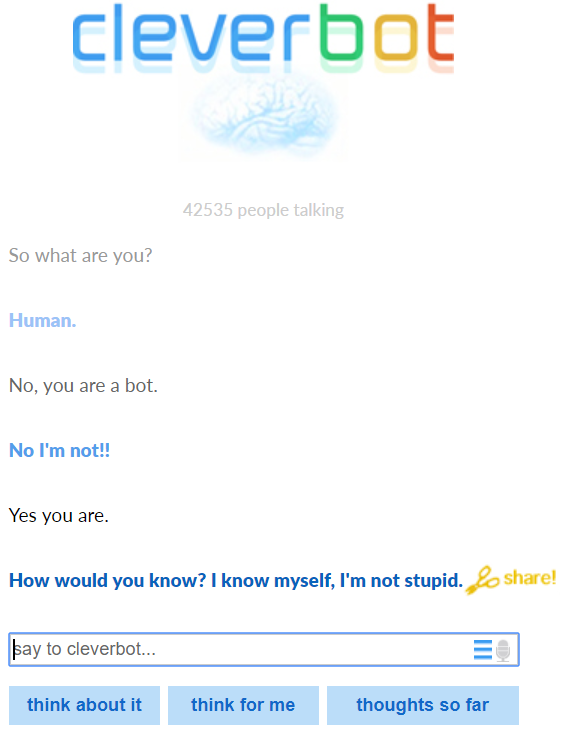
\includegraphics[width=0.4\textwidth]{pics/cleverbot.png}
	\caption{Sample conversation with Cleverbot \cite{Cleverbot:2017}}
\end{figure}


These chatbot programs are very similar in their core, namely that they all use hand-written rules to generate replies. Usually simple pattern matching or keyword retrieval techniques are employed to handle the user's input utterance. Then rules are used to transform a matching pattern or a keyword into a predefined reply.
A simple example is shown below in AIML \cite{Marietto:2013}:\\
{\color{OliveGreen}\textless category\textgreater}

{\color{OliveGreen}\textless pattern\textgreater}What is your name?{\color{OliveGreen}\textless/pattern\textgreater}

{\color{OliveGreen}\textless template\textgreater}My name is Alice{\color{OliveGreen}\textless/template\textgreater}\\
{\color{OliveGreen}\textless/category \textgreater}\\
\\
Here if the input sentence matches the sentence written between the \textit{\textless pattern\textgreater} brackets the reply written between the \textit{\textless template\textgreater} brackets is outputted.\\
Another example is shown below where we make use of the \textit{star} symbol to replace words. In this case whatever word follows the word \textit{like} it will be present in the response at the position specified by the \textit{\textless star/\textgreater} token:\\
{\color{OliveGreen}\textless category\textgreater}

{\color{OliveGreen}\textless pattern\textgreater}I like *{\color{OliveGreen}\textless/pattern\textgreater}

{\color{OliveGreen}\textless template\textgreater}I too like {\color{OliveGreen}\textless star/\textgreater}.{\color{OliveGreen}\textless/template\textgreater}\\
{\color{OliveGreen}\textless/category \textgreater}\\

\subsection{The Encoder-Decoder Model} \label{ssec:23}
The main concept that differentiates rule-based and neural network based approaches is the presence of a learning algorithm in the latter case. An important distinction has to be made between traditional machine learning and deep learning which is a sub-field of the former. In my work I talk about deep learning methods applied to chatbots since neural networks have been the backbone of the field of conversational modeling and traditional machine learning methods are only rarely used as supplementary techniques.   

When applying neural networks to natural language processing (NLP) tasks we have to transform each word (symbol) into a numerical representation \cite{Bengio:2003}. This is done through word embeddings, which represent each word as a fixed size vector of real numbers. Word embeddings are useful because instead of handling words as huge vectors of the size of the vocabulary we can represent them in much lower dimensions. I talk about the vocabulary used in NLP tasks in more detail in Section~\ref{sssec:234}. The vector that represents each word can be regarded as a set of parameters and these parameters can be jointly learned with the neural network's parameters, or they can be pre-learned which I detail further in Section~\ref{sssec:pretrain}.

Instead of using hand-written rules deep learning models transform input sentences into replies directly by using matrix multiplications and non-linear functions that contain millions of parameters. We can further divide neural network based conversational models into two categories, retrieval-based and generative models. The former simply returns a reply from the dataset by computing the most likely response to the current input utterance based on a scoring function, which can be implemented as a neural network \cite{Cho:2014} or by simply computing the cosine similarity between the input utterance and candidate replies \cite{stalemate:2016}. Generative models on the other hand synthesize the reply one word at a time by computing probabilities over the whole vocabulary \cite{Sutskever:2014,Vinyals:2015}. There have also been approaches that integrate the two types of dialog systems by comparing a generated reply with a retrieved reply and determining which one is more likely to be a better response \cite{Song:2016}.

As with many other applications the field of conversational modeling has been transformed by the rise of deep learning. More specifically the encoder-decoder recurrent neural network (RNN) model (also called seq2seq \cite{Sutskever:2014}) introduced by \cite{Cho:2014} and its variations have been dominating the field. After talking about RNNs in Section~\ref{sssec:231} I present the seq2seq model in Section~\ref{sssec:232}. This model was originally developed for neural machine translation (NMT), but it was found to be suitable to \textit{translate} source utterances into responses within a conversational setting \cite{Shang:2015,Vinyals:2015}.

\subsubsection{Recurrent Neural Networks} \label{sssec:231}
A recurrent neural network (RNN) \cite{RNN:1988} is a neural network that can take as inputs a variable length sequence \(\bm{x}=(\bm{x}_1,...,\bm{x}_n)\), by unfolding itself over each input \(\bm{x}_i\) and generating a hidden state at each step \(\bm{h}=(\bm{h_1},...,\bm{h_n})\). At each step \(i\), the hidden state \(\bm{h}_i\) is updated by
\begin{equation} \label{eq231a}
\bm{h}_i=f(W\bm{h}_{i-1}+U\bm{x}_i)
\end{equation}
which is also called the unrolling of the network. \(W\) and \(U\) are matrices containing the weights (parameters) of the network. \(f\) here is a non-linear activation function which can be the hyperbolic tangent function for example. The vanilla implementation of an RNN is rarely used, because it suffers from the vanishing gradient problem which makes it very hard to train \cite{Hochreiter:1998}. Usually long short-term memory (LSTM) \cite{Hochreiter:1997} or gated recurrent units (GRU) \cite{Cho:2014} are used for the activation function. LSTMs were developed to combat the problem of long-term dependencies that vanilla RNNs face. As the number of steps of the unrolling increase it becomes increasingly hard for a simple RNN to learn to remember information seen multiple steps ago. 

LSTM networks use a gating mechanism to control the information flow in the recurrent network. More specifically the input and forgetting gates are used to determine how to update the network's state and the output gate is used to determine what to output. Mathematically these gates consist of several matrix multiplications and non-linear functions applied to the input vector and the previous hidden state. LSTMs are particularly useful for language modeling, because we need to preserve information over multiple sentences while the network is unrolled over each word. Because of space constraints I don't detail LSTMs here further, but a very good quick explanation can be found in \cite{LSTM_article}. An important characteristic of recurrent neural networks is that the parameters of the function \(f\) don't change during the unrolling of the network.

\begin{figure}[H]
	\label{fig:231}
	\centering
	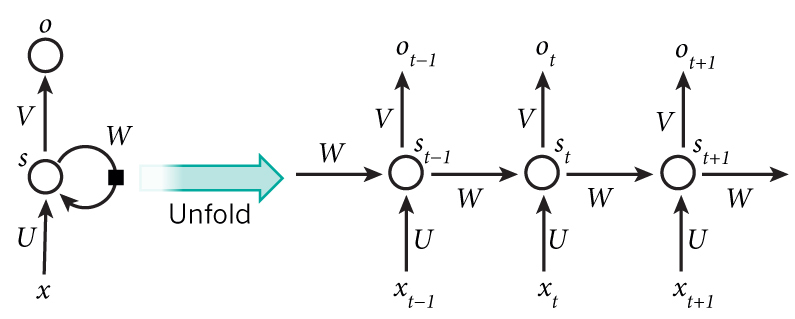
\includegraphics[width=0.5\textwidth]{pics/rnn.jpg}
	\caption{Unfolding of an RNN over 3 time-steps. Here \(x\) is the input sequence, \(o\) is the output sequence, \(s\) is the sequence of hidden states and \(U\),\(W\) and \(V\) are the weights of the network. \cite{RNN_pic:2017}}
\end{figure}

Language modeling is the task of predicting the next word in a sentence based on the previous words \cite{Bengio:2003}. RNNs can be used for language modeling by training them to learn the probability distribution over the vocabulary \(\bm{V}\) given an input sequence of words. As previously discussed the RNN receives the word embedding vectors representing words in lower dimensions. We can generate the probability distribution to predict the next word in the sequence by taking the hidden state of the RNN in the last step, and feeding it into a softmax activation function
\begin{equation} \label{eq231b}
p(\bm{x}_{i,j}|\bm{x}_{i-1},...,\bm{x}_1)=\frac{exp(\bm{v}_j\bm{h}_i)}{\sum_{j^{'}=1}^{K}exp(\bm{v}_{j^{'}}\bm{h}_i)}
\end{equation}
for all possible words (symbols) \(j=1,...,K\), where \(\bm{v}_j\) are the rows in the \(V\) weight matrix of the softmax function. \((\bm{x}_{i-1},...,\bm{x}_1)\) is the input sequence and \(\bm{h}_i\) is the hidden state of the RNN at step \(i\).

Training of these networks is done via the generalized backpropagation algorithm called truncated backpropagation through time \cite{Werbos:1990,RNN:1988}. Essentially we backpropagate the error through each time step of the network to learn its parameters. The error can be computed by using the cross-entropy loss, which calculates how different the predictions are compared to the true labels.
\begin{equation} \label{eq231c}
L(\bm{y}_i,\bm{\hat{y}}_{i})=-\bm{y}_i log(\bm{\hat{y}}_{i})
\end{equation}
where \(\bm{\hat{y}}_{i}\) is the vector of the predicted probabilities over all words in the vocabulary at step \(i\), and \(\bm{y}_i\) is the one-hot vector over the vocabulary. A one-hot vector is made up of zeros except at the index of the one true word that follows in the sequence, where it is equal to 1. After computing the derivative with respect to all of the weights in the network using the backpropagation through time algorithm we can update the weights in order to get closer to an optimum with optimization techniques like stochastic gradient descent (SGD) \cite{SGD:2010}. 

\subsubsection{The Seq2seq Model} \label{sssec:232}
The sequence to sequence model (seq2seq) was first introduced by \cite{Cho:2014}, but they only used it to re-rank sentences instead of generating completely new ones, which was first done by \cite{Sutskever:2014}. Since then, besides NMT and conversational models a plethora of different applications of these models have been introduced like text summarization \cite{Nallapati:2016}, speech recognition \cite{Chiu:2017}, code generation \cite{Rico:2017} and parsing \cite{Konstas:2017}, just to name a few.

\begin{figure}[H]
	\label{fig:232a}
	\centering
	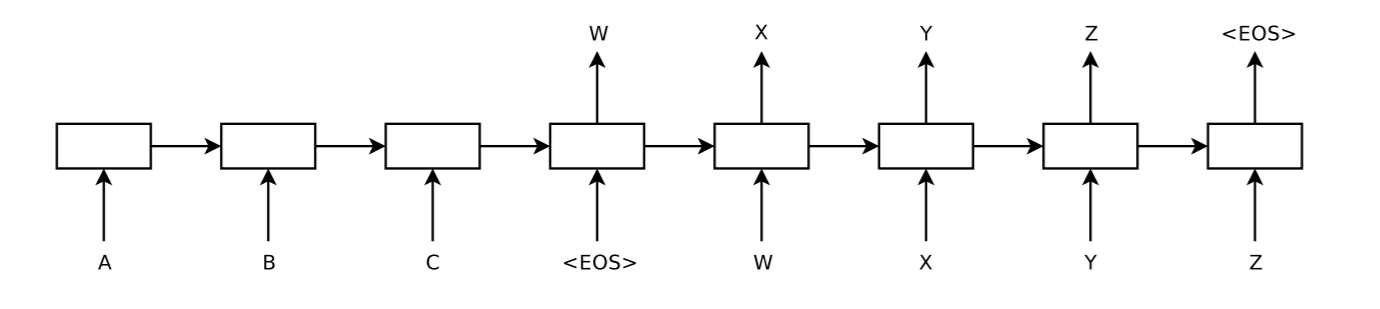
\includegraphics[width=0.9\textwidth]{pics/seq2seq.png}
	\caption{A general seq2seq model, where \((A,B,C)\) is the input sequence, \(<EOS>\) is a symbol used to delimit the end of the sentence and \((W,X,Y,Z)\) is the output sequence \cite{Sutskever:2014}}
\end{figure}

The simplest and initial form of the model is based on two RNNs. The actual implementation of RNNs can be in the form of LSTMs or GRUs as discussed in Section~\ref{sssec:231}. The goal is to estimate the conditional probability of \(p(\bm{y}_1,...,\bm{y}_{N^{'}}|\bm{x}_1,...,\bm{x}_N)\), where \(\bm{x}_1,...,\bm{x}_N\) is the input sequence and \(\bm{y}_1,...,\bm{y}_{N^{'}}\) is the corresponding output sequence. Since two different RNNs are used for the input and output sequences, the length of the sequences, \(N\) and \(N^{'}\) can be different. The encoder RNN is unrolled over the words in the source sequence and its last hidden state is called the thought vector, which is a representation of the whole source sequence. The initial hidden state of the decoder RNN is then set to this representation \(\bm{v}\), and the generation of target sequence words is done by taking the output of the unrolled decoder network at each time-step and feeding it into a softmax function, which produces the probabilities over all words in the vocabulary.
\begin{equation} \label{eq232a}
p(\bm{y}_1,...,\bm{y}_{N^{'}}|\bm{x}_1,...,\bm{x}_N)=\prod_{i=1}^{N^{'}}p(\bm{y}_i|\bm{v},\bm{y}_1,...,\bm{y}_{i-1})
\end{equation}

Training is very similar to a normal RNN, namely the log probability of a correct target sequence \(T\) given the source sequence \(S\) is maximized
\begin{equation} \label{eq232b}
\frac{1}{\bm{S}}\sum_{T,S \in \bm{S}}log(p(T|S))
\end{equation}
where \(\bm{S}\) is the training set. The two networks are trained jointly, errors are backpropagated through the whole model and the weights are optimized with some kind of optimization technique like SGD.

In NMT the input sequences are sentences in one language from which we wish to and target sequences are sentences in a different language to which we wish to translate. The individual elements of a sequence or sentence in this case are vectors representing word embeddings. In conversational modeling the simplest approach is to treat an utterance by a speaker as input sequence and the response to that utterance from a different speaker as the target sequence. I will talk about better approaches however in Section~\ref{sssec:context}.
\subsubsection{Deep Seq2seq Models}
Seq2seq models can also contain multiple layers of LSTM networks as seen in Figure~\ref{fig:232b}. This is done in order to make the model deeper and to have more parameters, which should ideally lead to better performance \cite{Vinyals:2015,googleNMT:2016}. There exist multiple variants, but the most straightforward one is to feed in the source sentence to the first layer of the encoder network. The output from the previous LSTM layer is fed as input to the next layer and the layers are unrolled jointly. Then the last hidden state of the final encoder layer can be used to initialize the initial hidden state of the first decoding layer. The output of the previous decoder layer is input to the next layer until the final layer, where we apply a softmax activation function over the outputs from the last layer to generate the predicted target sequence. How we initialize the layers in the decoder network can be implemented in many different ways, like taking the last hidden state from each encoder layer and using it to initialize the first hidden state of each corresponding decoder layer, to name another method.

\begin{figure}[H]
	\label{fig:232b}
	\centering
	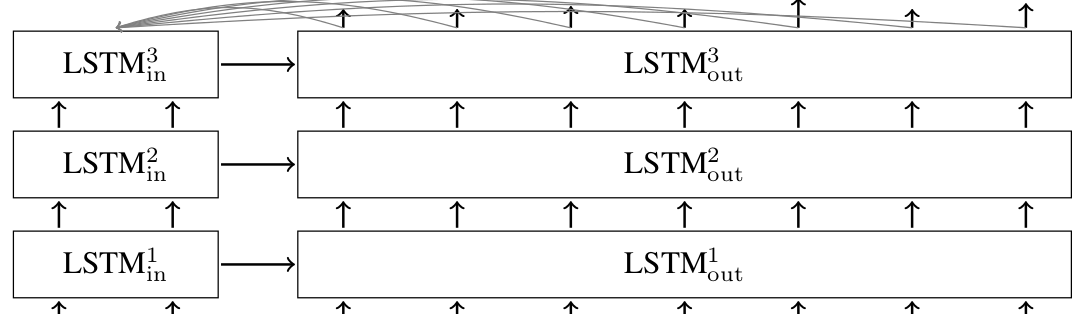
\includegraphics[width=0.55\textwidth]{pics/deep_seq2seq.png}
	\caption{A 3 layer seq2seq model \cite{deep_seq2seq}. The lines pointing from the last decoder states to the last encoder represent an attention mechanism about which I talk in Section~\ref{sssec:attention}}
\end{figure}

\subsubsection{Decoding and Vocabulary} \label{sssec:234}
In order to get the actual generated output sequences there are several techniques to decode from the probabilities of the words. One such technique is the Roulette Wheel selection, which is commonly used for genetic algorithms \cite{GA:1998}. Using this method, at each time-step each word from the vocabulary can be generated with the probability computed from the softmax function. This is useful if we want to have some stochasticity in the decoding process, because it can produce slightly different outputs for the same source sequence. However it doesn't perform as well as the more frequent method used, which is to simply output the word with the highest probability from the softmax function. This is a greedy and deterministic approach since we will always get the same output for the same input.

While decoding a word at each time-step is fine a better approach is to the decode the whole output sequence at the same time, by outputting the sequence with the highest probability.
\begin{equation} \label{eq233}
\hat{T}=\arg\max_{T}p(T|S)
\end{equation}
Here \(S\) is the source sentence and \(T\) is the target sentence. Since in order to get the sequence with the highest probability we have to first generate all of the possible sequences a simple left-to-right beam search is usually employed to make the computation tractable. First, \(K\) words with the highest probability are retained in the first time-step. Then at each time-step we expand this list by computing the joint probability of the partial sequences in the list and the words in the current time-step and retaining the \(K\) most probable partial sequences until we get to the end of the output sequence.

Another important aspect of sequence-to-sequence models applied to tasks involving language is the vocabulary. The vocabulary consists of all the different words and symbols present in the dataset. One problem with this approach is that the vocabulary tends to be quite large, especially for very big datasets like \cite{OpenSubtitles:2016,opensubtitles}. Since the number of parameters of the model increases proportionally with the size of the vocabulary it is usually the case that the vocabulary is limited to some arbitrary size \(K\). This way we only use the embeddings of the \(K\) most frequent words in the dataset and replace any other symbols with a common token representing unknown words. Many approaches have been proposed to the problem of handling out of vocabulary (OOV) or unknown words \cite{Luong:2014,Feng:2017,Jean:2014}. Other methods involve using characters \cite{Zhu:2017} or subword units \cite{Sennrich:2015} instead of words.

\newpage\section{Background} \label{sec:background}
In this section I will first present selected publications from my literature research. I categorize these papers into several categories, each corresponding to a specific approach or aspect of conversational modeling. In Section~\ref{ssec:31} I describe further details regarding encoder-decoder models and in Section~\ref{ssec:32} I give an overview of several techniques used to augment the performance of encode-decoder models. In Section~\ref{ssec:33} I present different approaches to conversational modeling that aren't based on the original seq2seq model.

Finally, in Section~\ref{ssec:problems} I present some criticism regarding basic techniques used in neural conversation models. While they are widely used, I show that the assumptions on which their usage rests are generally wrong and  in consequence these methods are unsuitable for modeling conversations. Finally I provide a brief summary of the section.

\subsection{Further Details of Encoder-Decoder Models} \label{ssec:31}
In this section I describe some further details regarding seq2seq models. First, I talk about the context of conversations and how it can be taken into account in Section~\ref{sssec:context}. Then I present different objective functions that can be used to train seq2seq models in Section~\ref{sssec:functions}. Finally I describe methods used for evaluating conversational agents in Section~\ref{sssec:eval}.

\subsubsection{Context} \label{sssec:context}
% In context section talk about simply feeding the whole conversation to encoder
In this section I first describe a commonly used variation of the RNN called the bidirectional RNN (BiRNN) \cite{Schuster:1997}. A BiRNN consists of two RNNs, a forward and a backward one. The forward RNN reads the input sequence in the original order (from \(\bm{x}_1\) to \(\bm{x}_n\)) and computes a sequence of forward hidden states \((\overrightarrow{\bm{h}}_1,...,\overrightarrow{\bm{h}}_n)\). The backward RNN reads the reversed sequence (from \(\bm{x}_n\) to \(\bm{x}_1\)) and computes the backward hidden states \((\overleftarrow{\bm{h}}_1,...,\overleftarrow{\bm{h}}_n)\). Then we can simply concatenate the two hidden states for each word in the sequence \cite{Bahdanau:2014,Zhaob:2017}. The BiRNN resembles a bag of words model, because each concatenated hidden state \(\bm{h}_i\) has information about the words surrounding the \(i\)-th word. This results in a better preservation of context and is used in several seq2seq models, usually in the encoder network \cite{Zhaob:2017,Xing_topic:2017,googleNMT:2016,Yin:2017}.
\begin{figure}[H]
	\label{fig:context}
	\centering
	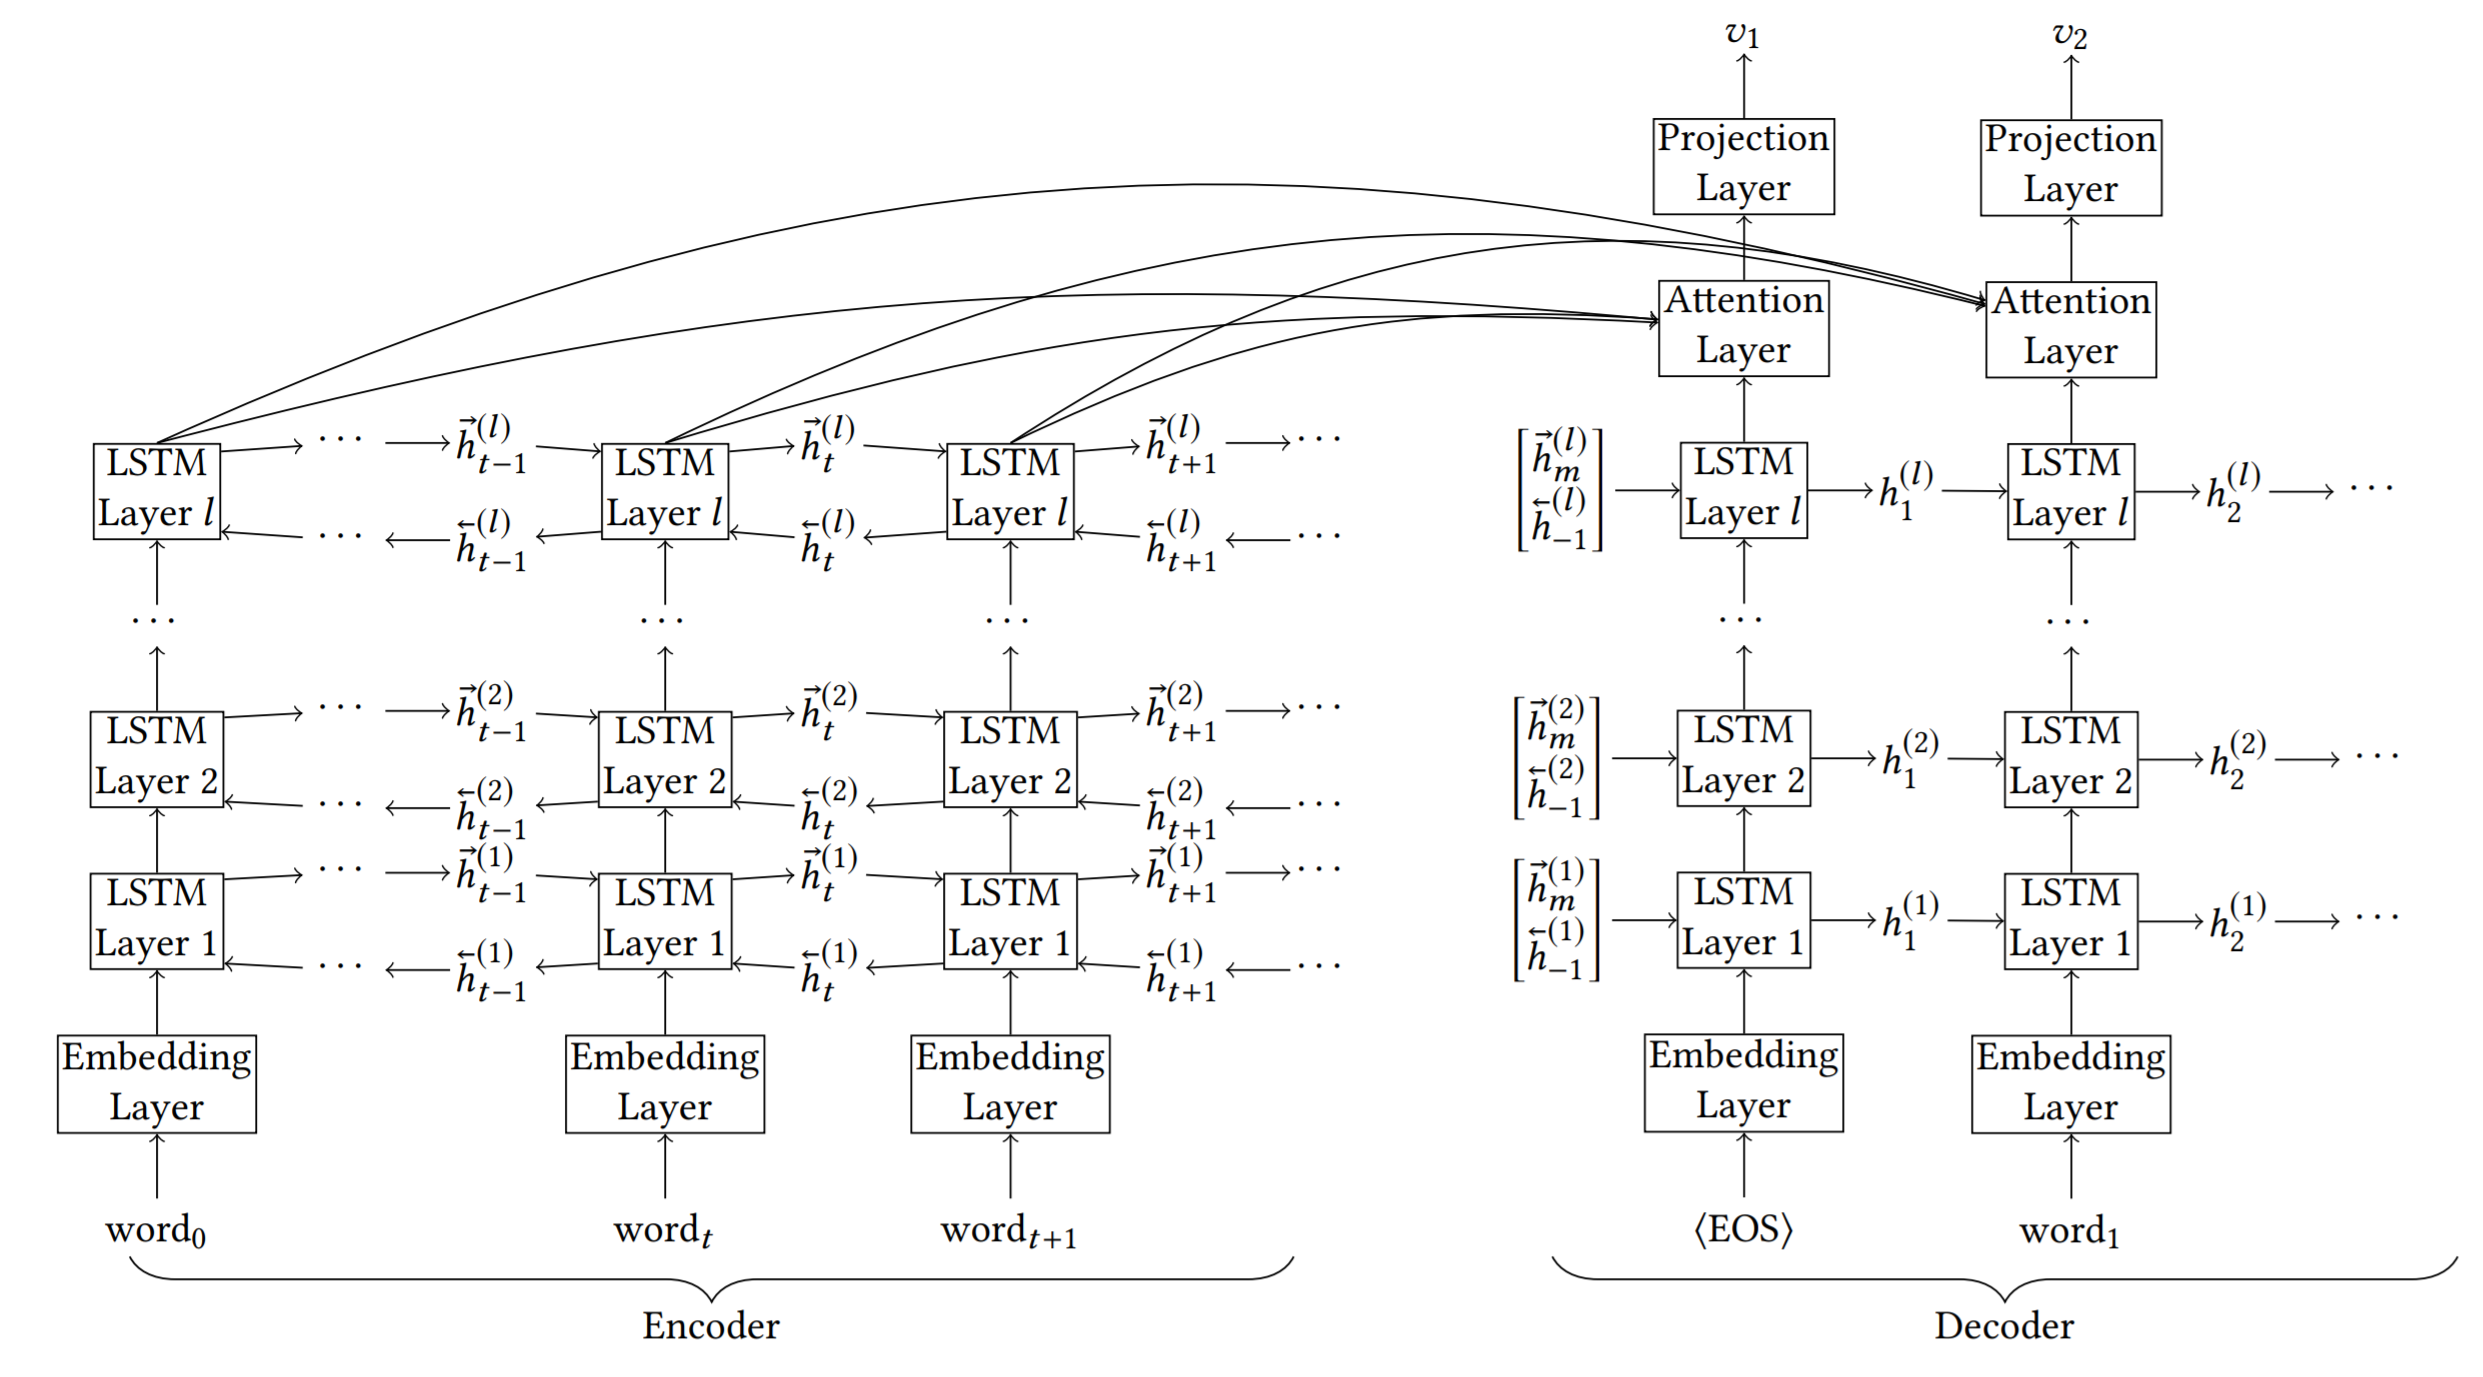
\includegraphics[width=1.0\textwidth]{pics/bilstm.png}
	\caption{A bidirectional multilayer LSTM encoder and unidirectional LSTM decoder with attention \cite{Yin:2017}}
\end{figure}
So far I have only described conversational modeling as predicting a reply based on a single source utterance. However conversations are more complicated than machine translation, since they don't solely consist of utterance-reply pairs. Conversations usually have many turns, and the reply to an utterance might depend on information presented in previous turns of the conversation. A plethora of approaches have been proposed to incorporate context or conversation history into seq2seq models in order to build better dialog agents. Perhaps the most straightforward approach is to concatenate \(k\) previous utterances by appending an end-of-utterance symbol after each utterance and feeding this long sequence of symbols into the encoder \cite{Vinyals:2015}. The simplest approach which was used as a baseline in \cite{Sordoni:2015} is to use only the first preceding utterance as context in order to form context-message-reply triples for training. A better approach was to concatenate the bag of words representations of the context and message utterances instead of the actual utterances. By using different representations for different utterances better results were achieved \cite{Sordoni:2015}.

However feeding long sequences of symbols into the encoder RNN of seq2seq models accentuates the vanishing gradient problem \cite{Hochreiter:1998}. Also as sequences get longer it becomes increasingly more difficult for RNNs to retain information which was inputted many time-steps ago. Consequently, it becomes even harder to encode all relevant information into the last hidden state of the encoder network from a sequence consisting of multiple sentences.

A possible solution is to represent the current utterance and previous dialog turns with different RNNs and to build a hierarchical representation of the conversation history \cite{Serban:2015}, which I describe in detail in Section~\ref{sssec:HRED}. A similar approach was presented in \cite{Zhaob:2017} using one RNN to encode the current utterance and a different RNN to encode \(k\) previous utterances, but this approach doesn't take into consideration the hierarchical nature of conversations.
 

\subsubsection{Objective Functions} \label{sssec:functions}
In addition to the standard cross-entropy loss introduced in Section~\ref{sssec:231} there have been proposed several different loss functions for conversational models in order to generate more varied and interesting replies. One such class of loss functions are reinforcement learning based, which I talk about in detail in Section~\ref{sssec:RL}. In \cite{Ramachandran:2016} a seq2seq model is pretrained as a language model and in order to avoid over-fitting monolingual language modeling losses are added to the standard loss function. These losses act as a regularizer by forcing the seq2seq model to correctly model both the normal seq2seq task and the original monolingual language modeling tasks. I talk about pretraining in more detail in Section~\ref{sssec:pretrain}. In \cite{Lison:2017} it is argued that not all context-response pairs in a dialog dataset have the same importance for conversational modeling. Accordingly they weight each context-response pair with a scoring model and use these weights in the loss function when training a seq2seq model. Hence, examples associated with bigger weights in the dataset will have a larger impact on the gradient update steps through the loss function. 

Approaches to incorporate beam search into the training procedure have also been explored. In \cite{Wiseman:2016} a simple approach is taken to construct the loss function by penalizing when the gold target sequence is not present in the beam consisting of the most likely predictions. The issue with incorporating beam search directly into the training procedure of seq2seq models is that it uses the argmax function which is discontinuous and hence is not amenable to backpropagation. Since the predictions, which serve as input to the standard loss function are discrete (from beam search), the evaluation of the final loss is also discontinuous. A relaxation based technique is proposed in \cite{Goyal:2017}, where the beam search based loss function is gradually relaxed to the standard loss function as training progresses.

Perhaps the most extensively used objective function besides the standard one is based on Maximum Mutual Information (MMI) \cite{Li:2015}. In MMI the goal is defined as maximizing pairwise or mutual information between a source sentence \(S\) and the corresponding target \(T\):
\begin{equation}
\log{\frac{p(S,T)}{p(S)p(T)}}=\log{p(T|S)}-\log{p(T)}
\end{equation}
By introducing a weighting constant \(\lambda\) and by using the Bayes' theorem the training objective can be written in the following two ways:
\begin{equation} \label{eqMMIa}
\hat{T}=\arg\max_{T}[\log{p(T|S)}-\lambda\log{p(T)}]
\end{equation}
\begin{equation} \label{eqMMIb}
\hat{T}=\arg\max_{T}[(1-\lambda)\log{p(T|S)}+\lambda\log{p(S|T)}]
\end{equation}
However, it is not trivial to use these equations as loss functions in practice. In Equation~\ref{eqMMIa} the term \(\lambda\log{p(T)}\) acts as an anti-language model since it is subtracted from the loss function. This leads to ungrammatical output sentences in practice. Training using Equation~\ref{eqMMIb} is possible since we just have to train an additional seq2seq model for the \(\log{p(S|T)}\) term by using targets as inputs and inputs as targets, but direct decoding is intractable since it requires completion of target generation before \(p(S|T)\) can actually be computed. Solutions to these issues have been proposed in \cite{Li:2015}.

\subsubsection{Evaluation Methods} \label{sssec:eval}
Evaluation of dialog systems is perhaps a more controversial topic. Indeed it is still an open research problem to find good automatic evaluation metrics that can effectively compare the performance of conversational models. The traditional approach is to use the same metrics that are used for NMT and language modeling. Bleu and perplexity are widely used metrics for evaluating dialog systems \cite{Vinyals:2015,Yao:2016,Zhao:2017,Serban:2015}. 

Bleu \cite{Papineni:2002} measures how many n-word-sequence (n is usually 4) overlaps are there between the test sentences and the predicted ones by the model. Similar to this but less commonly used is the simple accuracy of the whole sentence or the word error rate, which is prevalent for speech recognition models \cite{Shannon:2017,Park:2008} and calculates how many words are incorrect in the predicted sentence.

Perplexity \cite{Manning:1999} is another common metric, which measures how well a probability model predicts a sample. Given a model we can plug sentences that it hasn't seen during training and compute the perplexity on the test set. If we have a model \(q\) (encoder-decoder for conversational modeling), we can compute the perplexity by
\begin{equation}
2^{-\frac{1}{N}\sum_{i=1}^{N}\log_2{q(\bm{x}_i)}}
\end{equation}
where \(x_i\) are the test samples or words in the sentence and \(N\) is the length of the sentence. Essentially we want our models to give very high probability to test samples, meaning that the lower the perplexity score the better.

Unfortunately it has been shown that these metrics don't correlate well with human judgment in the conversational setting \cite{Liu:2016}. I talk about the downfalls of these standard metrics in Section~\ref{sssec:metrics}. A number of different methods have been proposed to address the problem of evaluating conversational agents, for example how many turns it takes until the model produces a generic answer \cite{Zhao:2017,Li_RL:2016} or the diversity of the generated responses \cite{Li_RL:2016}. More sophisticated metrics make use of neural network based models to assign a score to utterance-response pairs and it has been shown that they correlate better with human judgments than traditional metrics \cite{Lowe:2017,Tao:2017}.

For reinforcement learning and task-oriented dialog agents, which I describe in Section~\ref{sssec:RL} and Section~\ref{sssec:task} respectively evaluation is more straightforward. In reinforcement learning we specify a goal that the dialog agent has to achieve, and we can simply measure its performance based on the percent of cases in which it achieves the goal \cite{Li_adversarial:2017,Havrylov:2017}. Similarly for task-oriented dialog agents usually there is a clearly defined task and the accuracy of accomplishing the given task serves as a good performance metric \cite{Joshi:2017,Zhao:2017,Li_HIL:2016}.

Finally, one of the better methods to evaluate dialog systems is to ask other people what they think about the quality of the responses that an agent produces. Human judgment has been one of the most prevalent metrics throughout recent literature related to conversational modeling \cite{Shang:2015,Vinyals:2015,Zhou:2017,Li_RL:2016,Zhao:2017,Li_RL:2016,Li:2015}. Usually human judges are asked to either rate the quality of individual responses from a model on a scale or to choose the better response from responses produced by different models for the same input. A number of properties of conversations can be rated, like naturalness, grammaticality, engagement or simply the overall quality of the conversation.

\subsection{Augmentations To The Encoder-Decoder Model} \label{ssec:32}
In this section I present recent methods and techniques used to augment the performance of encoder-decoder models. In Section~\ref{sssec:attention} I describe different attention mechanisms. Furthermore I show how pretraining of seq2seq models can help in a conversational setting in Section~\ref{sssec:pretrain}. Then I talk about different features and priors that can be used as additional inputs to seq2seq models in Section~\ref{sssec:priors}. Finally I show how knowledge bases and information retrieval can be good additions to encoder-decoder models in Section~\ref{sssec:KB}.

\subsubsection{Attention} \label{sssec:attention}
% max mention attention is all you need here, because it will be described in ssec:41
The attention mechanism was first introduced to encoder-decoder models by \cite{Bahdanau:2014}. The problem that it was trying to address is the limited information that the context vector can carry. In a standard seq2seq model we expect that this single fixed-size vector can encode all the relevant information about the source sentence that the decoder needs in order to generate its prediction. Additionally, since we use a single vector, all the decoder states receive the same information, instead of feeding in information relevant to the specific decoding step. 


\begin{figure}[H]
	\label{fig:attentiona}
	\centering
	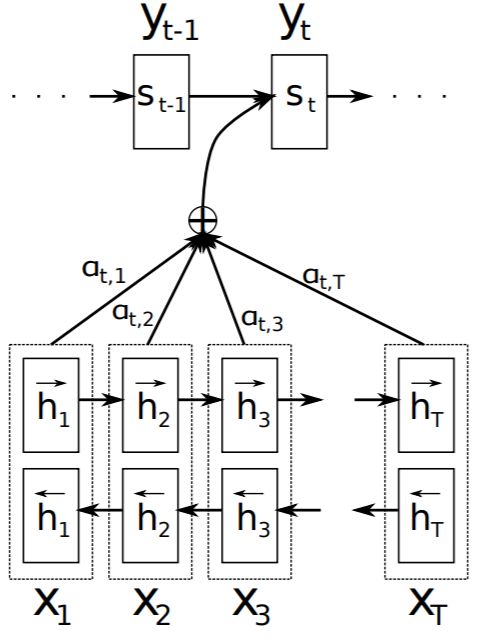
\includegraphics[width=0.3\textwidth]{pics/bahdanau_attn.png}
	\caption{Original Attention Mechanism \cite{Bahdanau:2014}}
\end{figure}
In order to combat these shortcomings the attention mechanism creates an additional input at each decoding step coming directly from the encoder states. This additional input \(\bm{c}_i\) to the decoder at time-step \(i\) is computed by taking a weighted sum over the encoder hidden states \(\bm{h}\):
\begin{equation} \label{eqattention}
\bm{c}_i=\sum_{j=1}^{T}a_{ij}\bm{h}_j
\end{equation}
where \(T\) is the number of hidden states or symbols in the source sentence and the weight \(a_{ij}\) for each \(\bm{h}_j\) hidden state can be computed by
\begin{equation}
a_{ij}=\frac{exp(e_{ij})}{\sum_{k=1}^{T}exp(e_{ik})}
\end{equation}
which is basically a softmax function over \(e_{ij}\), which is the output of a scoring function:
\begin{equation}
e_{ij}=f(\bm{s}_{i-1},\bm{h}_j).
\end{equation}
Here \(\bm{s}_{i-1}\) is the hidden state of the decoder in the previous time-step. Oftentimes \(\bm{s}_{i-1}\) is called a query vector \(\bm{q}\) and the encoder hidden states \(\bm{h}\) are called key vectors \(\bm{k}\).
The scoring function \(f\) can be implemented in several ways:
\begin{equation}
MLP(\bm{q},\bm{k})=\bm{w_2}tanh(W_1[\bm{q}:\bm{k}])
\end{equation}
where we simply concatenate the query and key vectors and feed them into a single or multilayer neural network \cite{Bahdanau:2014}. \(\bm{w}_2\) and \(W_1\) are the weights of the network.
\begin{equation}
BL(\bm{q},\bm{k})=\bm{q}^\mathsf{T}W\bm{k}
\end{equation}
is called the bilinear scoring function where \(W\) is a learned weight matrix. \cite{Luong:2015}.
\begin{equation}
DP(\bm{q},\bm{k})=\bm{q}^\mathsf{T}\bm{k}
\end{equation}
is the dot product scoring function, which doesn't use any weights, but it requires the sizes of the two vectors to be the same \cite{Luong:2015}.
\begin{equation}
SDP(\bm{q},\bm{k})=\frac{\bm{q}^\mathsf{T}\bm{k}}{\sqrt{|\bm{k}|}}
\end{equation}
is the scaled dot product, where we scale the previous dot product by the square root of the size of the key vectors \cite{Vaswani:2017}. This is useful because otherwise the dot product increases as dimensions get larger.

We can attend to outputs from the decoder network generated in previous time-steps by incorporating them as additional inputs to the scoring functions mentioned above \cite{Shao:2017}. This helps the decoder by allowing it to \textit{see} what has already been generated.

Attention can also be implemented using multiple heads \cite{Vaswani:2017}, meaning that we use the output of multiple scoring functions, each with their own parameters to learn to focus on different parts of the input sequence. The parameters of the scoring functions are jointly learned with all other parameters of the seq2seq model.



\begin{figure}[H]
	\label{fig:attentionb}
	\centering
	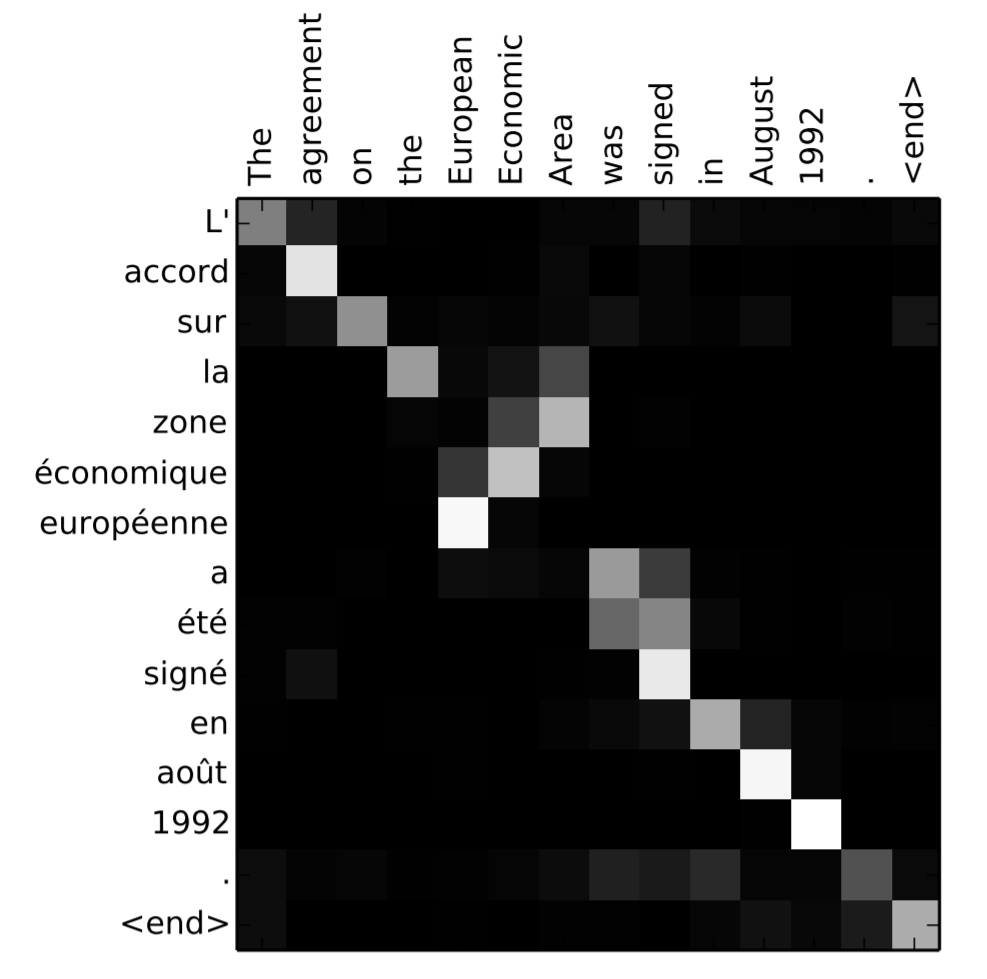
\includegraphics[width=0.4\textwidth]{pics/attn_weights.png}
	\caption{Pixels represent the weights \(a_{ij}\) between inputs and outputs \cite{Bahdanau:2014}}
\end{figure}
Attention can also be computed using only one sequence of symbols \cite{Cheng:2016,Lin:2017,Vaswani:2017}. In this case the query and key vectors both come from the same hidden states and thus we get an encoding of the sentence which depends on all of its parts. This is called self or intra-attention and it can be used both in the decoder and the encoder networks since it can be implemented as a standalone layer that takes in a sequence and computes a new representation of that sequence. 
\begin{figure}[H]
	\label{fig:attentionc}
	\centering
	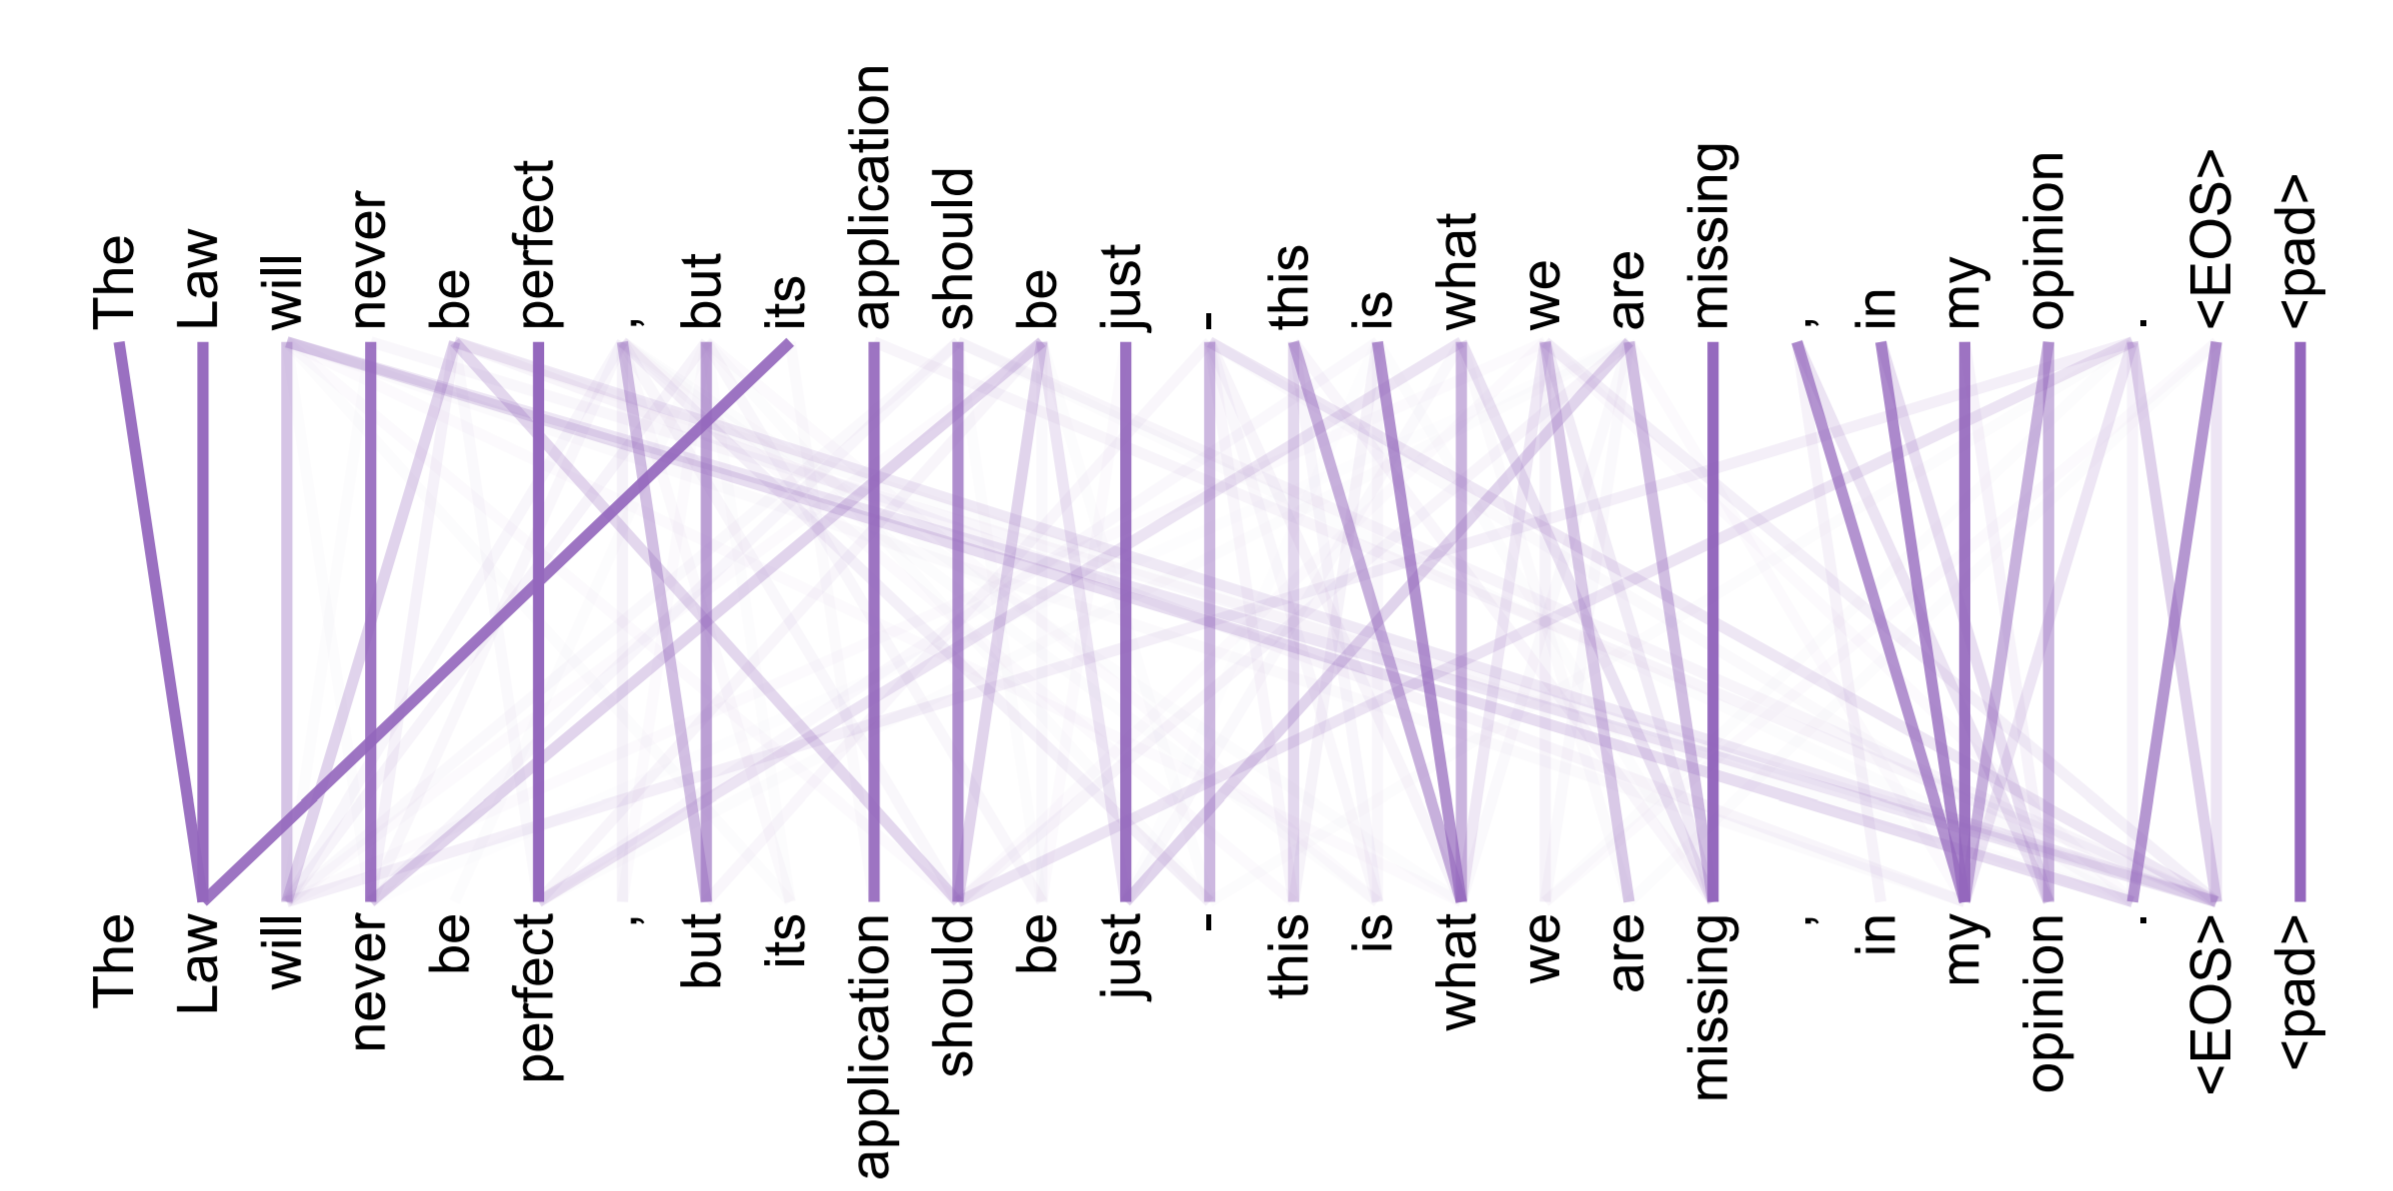
\includegraphics[width=0.7\textwidth]{pics/self_attn.png}
	\caption{Visualizing self-attention, lines represent the weights \(a_{ij}\) \cite{Vaswani:2017}}
\end{figure}

Attention has been extensively used for neural conversation models as an augmentation of the base seq2seq model \cite{Yao:2016,Shang:2015,Xing_topic:2017,Zhao:2017}. A more complex type of attention mechanism is the hierarchical attention which was used in conversational modeling \cite{Xing:2017} and abstractive text summarization \cite{Nallapati:2016} as well. It is useful when we need to attend over multiple input sentences. I describe it in more detail in Section~\ref{sssec:HRED}.

\subsubsection{Pretraining} \label{sssec:pretrain}
Pretraining for seq2seq models means that instead of initializing the parameters of a model randomly we pretrain the model on some data or some other task that is different from the main task that we want to apply our model to. One of the most common approaches among many NLP tasks is to pretrain the parameters of the word embeddings \cite{Chen:2014,Serban:2015,Akasaki:2017,Lample:2016,Serban:2017}. The most popular techniques to pretrain word embeddings are presented in these papers \cite{Mikolov:2013,Mikolov_skipgram:2013}. An advantage of pretraining word embeddings is that during the actual training of the seq2seq model we can fix these embeddings and thus the model has to learn less parameters. The reason why this works in practice is that word embeddings are just representations of words, hence these parameters don't take an active part in task specific learning, like NMT or conversational modeling.

In addition to pretraining word embeddings we can also pretrain all of the parameters of an encoder-decoder model. For conversational modeling this is very beneficial, because oftentimes well labeled datasets are relatively small. By pretraining on a big but noisier dataset the parameters of the model will already achieve somewhat good performance. Thus the model will have learned a good amount of general knowledge about the task \cite{Li:2016,Serban:2015}. Then by finetuning on the smaller dataset it can achieve better performance without overfitting this smaller dataset. For example a conversational model can learn general knowledge like answering with yes or no to a yes or no question. Then during finetuning the model doesn't have to learn all of this knowledge again and thus can focus on more subtle properties of conversation or domain-specific knowledge. In \cite{Li:2016} a seq2seq model was pretrained on the OpenSubtitles dataset \cite{OpenSubtitles:2016} and then adapted the pretrained model to a much smaller TV series dataset. A somewhat different approach was employed in \cite{Ramachandran:2016}, where the authors pretrained the encoder and decoder RNNs of a seq2seq model separately as language models. Thus both networks already had some knowledge about language before putting them together and training the whole seq2seq model for NMT. Similarly in \cite{Sriram:2017} a pretrained language model (LM) was used to augment the performance of standard seq2seq model. With the information from the LM the seq2seq model was able to improve its performance for domain adaptation, which means that it performed almost as good on a different domain as on the domain it was trained on.

In \cite{Lowe:2017} the authors made an attempt at building a model which automatically assigns scores to sample conversations. To do this they used the encoder and context RNN part of a HRED network (which I talk about in Section~\ref{sssec:HRED}) to encode the conversation. Since their dataset of scored conversations was small they resorted to pretrain the HRED with the normal task of generating replies to conversations.

Lastly, a different style of pretraining was employed in \cite{Wiseman:2016}. Instead of pretraining a seq2seq model with a different dataset they pretrained the model with a different loss function. This was necessary since the authors tried to integrate beam search into the loss function, but found that without first pretraining with the standard cross-entropy loss function the model was unable to learn anything with their new loss function.

\subsubsection{Additional Input Features} \label{sssec:priors}
In addition to the raw dialog turns we can integrate a plethora of other inputs into the seq2seq model. A number of attempts have been made since the birth of the encoder-decoder model in order to augment it with additional input features. The goal of these features is mainly to provide more information about the conversation or the context. In addition, models infused with additional features can learn to differentiate between different styles of dialog. By conditioning a seq2seq model on speaker information it can learn to output replies in the style of the speaker it was trained on \cite{Li:2016}. In this paper the authors input additional speaker embeddings into the decoder. These speaker embeddings are similar to word embeddings, basically representing the speakers for the utterances in the dataset. The additional speaker embedding vector is fed into the decoder RNN at each time-step jointly with the previously generated word. The result is a more consistent conversational model. Because of the speaker embeddings it learns general facts associated with the specific speaker. For example to the question \textit{Where do you live?} it might reply with different answers depending on the speaker embedding that is fed into the decoder. Additionally the authors have also experimented with speaker-addressee models. This is a simple extension to the previously discussed speaker model. Instead of simply feeding in speaker embeddings to the decoder RNN a weighted sum of the speaker and addressee embeddings is inputted. The addressee is the speaker to which the utterance is directed. The intuition behind this addition is that we talk in different styles depending on who we talk to (boss, friend, lover). Thus, the model not only responds differently with different speaker embeddings but it also conditions its response on the addressee embeddings. Hence, it might output a different reply for the same utterance and speaker embedding but different addressee embedding.

\begin{figure}[H]
	\label{fig:persona}
	\centering
	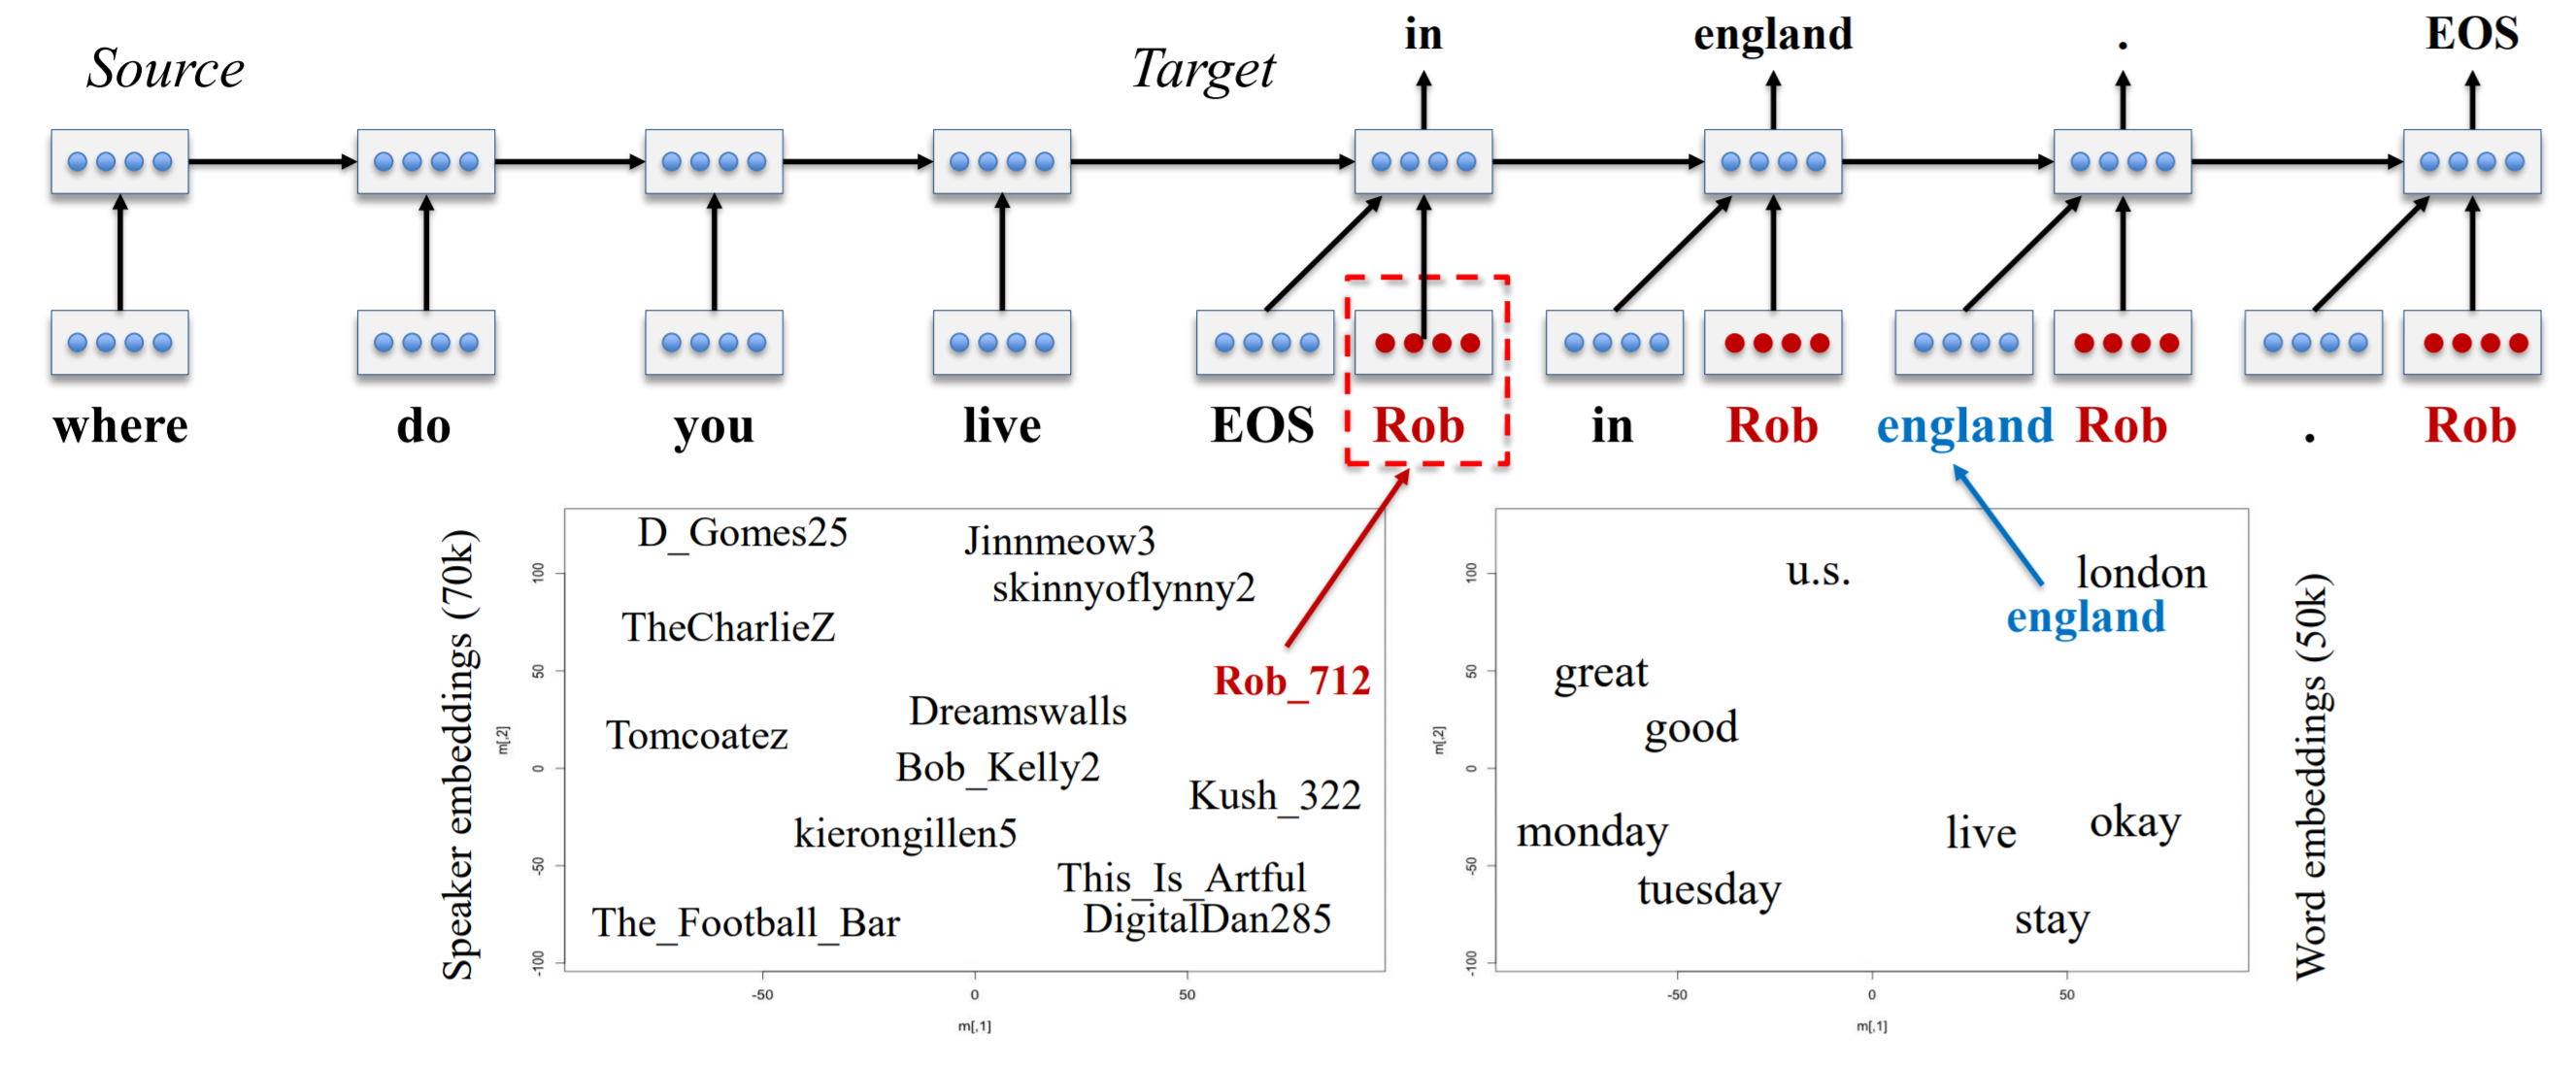
\includegraphics[width=0.9\textwidth]{pics/persona.png}
	\caption{A seq2seq model augmented with speaker embeddings \cite{Li:2016}}
\end{figure}

Similarly to this many other approaches were made to condition the response generation on various types of categories. For example in \cite{Xing_topic:2017} topic words are extracted from each utterance in the dataset. Then a seq2seq model is trained with these additional topic words together with the utterance they belong to. More specifically a separate attention mechanism is implemented that attends over the topic words. The two vectors generated from the normal utterance attention and the topic attention are fed into the decoder RNN at each time-step. With this additional topic information the model manages to produce more relevant replies to the topic of the conversation. A somewhat different approach to include topic information into the response generation process was employed in \cite{Choudhary:2017}. In this work three seq2seq models were trained separately on three datasets related to different topics (domains). Additionally a domain classifier based on logistic regression was trained to compute the probability that the utterance is related to a domain for all three domains. At test time, for an input utterance all the seq2seq models generate a reply and the domain classifier predicts a domain. Then a re-ranker takes the generated responses and the predicted domain probabilities and multiplies them together to determine the most probable reply-domain pair. Another example involves using emotion categories for post-response pairs \cite{Zhou:2017}. Here the authors first classify all of the post-response pairs in the dataset with an LSTM model into several emotion categories like happy, sad, angry, etc. Then they feed in these categories as real-valued vector representations into the decoder of an encoder-decoder model during training. Additionally a more complex memory based augmentation is proposed to the encoder-decoder model to better capture emotional changes in the response, which I don't detail here. In essence by feeding in these emotion categories we can generate a reply conditioned on a specific type of emotion. For example the response for the question \textit{How was your day?} will differ in style for different emotion categories.

A different approach is taken in \cite{Ghazvininejad:2017}, where the emphasis is put on taking into account relevant facts to an utterance. A seq2seq model is upgraded with a fact encoder which operates over a knowledge base which stores facts about different locations (eg. restaurants, theaters, airports). Before generating the reply to an encoded utterance a location or entity is extracted from it with keyword matching or named entity recognition. Then based on the location or entity, relevant facts are selected from the knowledge base, which are encoded by a memory network \cite{Sukhbaatar:2015}. Afterwards the vector representation from the encoded facts and the vector representation from the encoded utterance are summed and fed into the decoder RNN of the encoder-decoder model which generates the response. The authors used Twitter post-reply-reply 3-turn conversations which included a handle or hashtag about locations for which relevant facts were selected from a knowledge-base. With this approach the conversational model managed to produce more diverse and relevant replies if there was a location identified in the source utterance. Other similar methods involve leveraging information from knowledge bases as additional inputs which I describe in detail in Section~\ref{sssec:KB}. 

Other approaches try to integrate more features into the seq2seq model without using additional information. In a standard seq2seq model the only information the model has about the source utterance is through the vector representations of the words. To enrich the representation of the natural language utterance many other features have been proposed to be fed into the encoder RNN together with the word embeddings \cite{Sordoni:2015, Serban_MrRNN:2017,Serban:2017}. Such features include part-of-speech tags, dialog acts and n-gram word overlaps, just to name a few.

\subsubsection{Knowledge Bases, Copying and Information Retrieval} \label{sssec:KB}
\subsection{Different Approaches to Conversational Modeling} \label{ssec:33}
In this section I first describe hierarchical models used for building conversation agents in Section~\ref{sssec:HRED}. Then I talk about some approaches to integrate task-oriented conversations and goals with encoder-decoder models in Section~\ref{sssec:task}. Furthermore I present reinforcement learning based approaches in Section~\ref{sssec:RL}, that have seen some success when applied to the task of training conversational agents. Finally, I present encoder-decoder models that are very different from the standard RNN based seq2seq in Section~\ref{sssec:diffencdec}, but nonetheless have achieved state-of-the-art results.

\subsubsection{Hierarchical Models} \label{sssec:HRED}
In order to better represent dialog history a general hierarchical recurrent encoder-decoder (HRED) architecture was presented in \cite{Serban:2015}. The model consists of three different RNNs, the encoder RNN, the context RNN and the decoder RNN. First, \(k\) previous utterances of a conversation are encoded separately by the encoder RNN. This produces \(k\) separate context vectors by taking the last hidden state of the encoder RNN from each encoded utterance. Then these \(k\) hidden states are fed into the context RNN step by step, thus the it has to be unrolled for \(k\) steps. Next, the last hidden state from the context is used to initialize the decoder RNN. The decoder RNN and the decoding process is very similar to the seq2seq model.

The HRED differs from the basic encoder-decoder model by introducing a new level of hierarchy, the context RNN, which computes hidden states over entire utterances. With this approach the natural hierarchy of conversations is preserved by handling word sequences with the encoder RNN and utterance sequences with the context RNN which depends on the hidden representations produced by word-level encoding.

\begin{figure}[H]
	\label{fig:HRED}
	\centering
	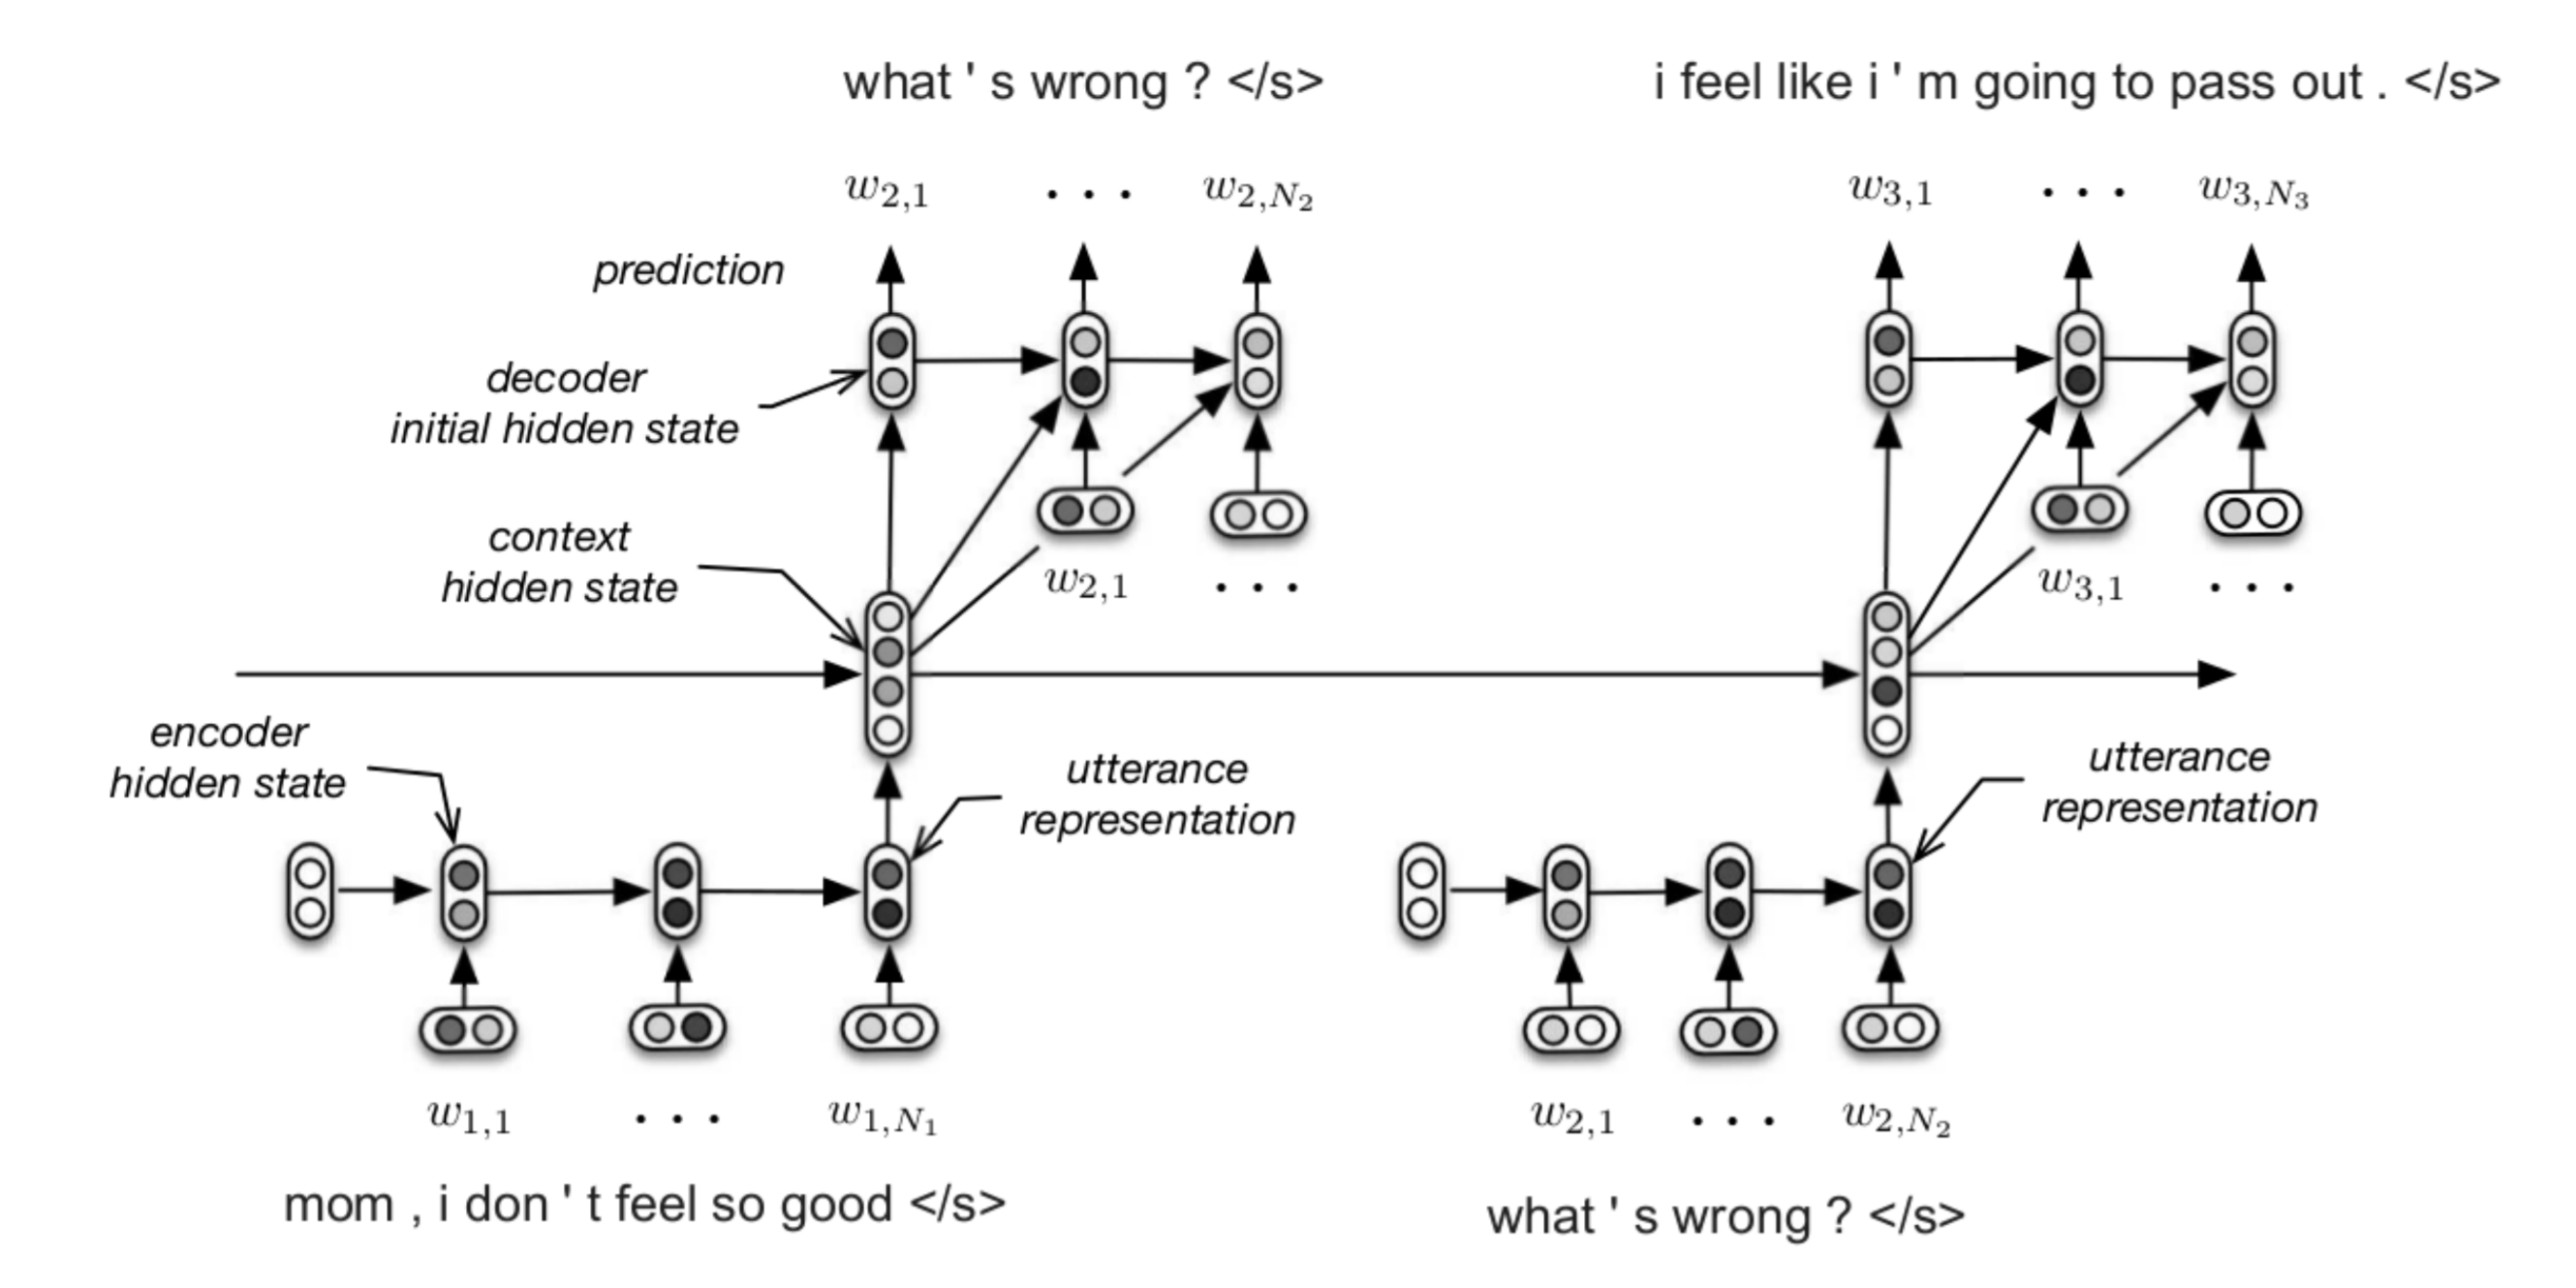
\includegraphics[width=0.9\textwidth]{pics/HRED.png}
	\caption{The Hierarchical Recurrent Encoder-Decoder Model \cite{Serban:2015}}
\end{figure}
Since the introduction of the HRED model a number of works have used and augmented it \cite{Serban_VHRED:2017,Serban_MrRNN:2017,Serban:2017,Shen:2017,Li_adversarial:2017}. A proposed extension to the HRED model is to condition the decoder RNN on a latent variable which is sampled from the prior distribution at test time and the approximate posterior distribution at training time \cite{Serban_VHRED:2017}. These distributions can be represented as a function of previous sub-sequences of words. 

In \cite{Serban_MrRNN:2017} two HRED models are employed simultaneously. One HRED operates over coarse tokens of the conversation (eg. POS tags) to generate coarse predictions. Then the second HRED which takes as input the natural language utterances generates natural language predictions by conditioning on the predicted coarse tokens. This conditioning is done via concatenating the last hidden state of the decoder RNN of the coarse predictions with the current context RNN hidden state from the natural language HRED and feed it into the natural language decoder RNN.

In order to handle the two-party style of conversations, two separate hierarchical recurrent encoder (HRE) models are used in \cite{Shen:2017}. The HRE is similar to the HRED, the only difference being that it misses the decoder RNN. One of the HRE networks encodes only the utterances coming from one of the speakers, and the other HRE encodes the utterances of the other speaker. Thus at each turn the two networks produce two hidden context states which are concatenated and fed into a single decoder RNN, which produces the output prediction.

A natural extension to the original HRED model is to incorporate attention mechanisms which was explored in several works \cite{Yao:2015,Yao:2016,Xing:2017}. The simplest form of integrating attention with the HRED model is between the previous decoder RNN hidden state and the encoder RNN hidden states from the previous turn. This can be done in exactly the same way as in standard seq2seq models and has been explored in \cite{Yao:2015,Yao:2016}.

A more interesting approach is to make use of the hierarchical structure of the HRED and integrate attention hierarchically as well \cite{Xing:2017}. Accordingly the model in this work is called the hierarchical recurrent attention network (HRAN). There are two levels of attention employed. The word level attention mechanism computes vector representations over the hidden states of the encoder RNN (keys) and the previous hidden state of the decoder RNN (queries). Each utterance is encoded separately by the encoder RNN and word level attention is also computed separately for each utterance. The produced vector representations are fed into the utterance level encoder (context RNN). Then the utterance level attention mechanism computes a context vector based on the hidden states of the context RNN. The last step is to feed in this context vector into the decoder RNN at each step, which computes the output sequence predictions. 

An additional technique employed in the HRAN architecture is to use context RNN hidden states as input to the word level attention. More specifically the context RNN is implemented in a reverse order, meaning that if we have a sequence of utterances \((u_1,...,u_n)\), the encoder RNN first encodes \(u_n\), thus the utterance level encoder will also start with the vector representation from the last utterance in the conversation. Because the utterances are reversed the word level attention mechanism for each utterance can use as additional input the hidden state of the context RNN from the next utterance in the original order. Figure~\ref{fig:HRAN} depicts the HRAN with all the components mentioned above.
\begin{figure}[H]
	\label{fig:HRAN}
	\centering
	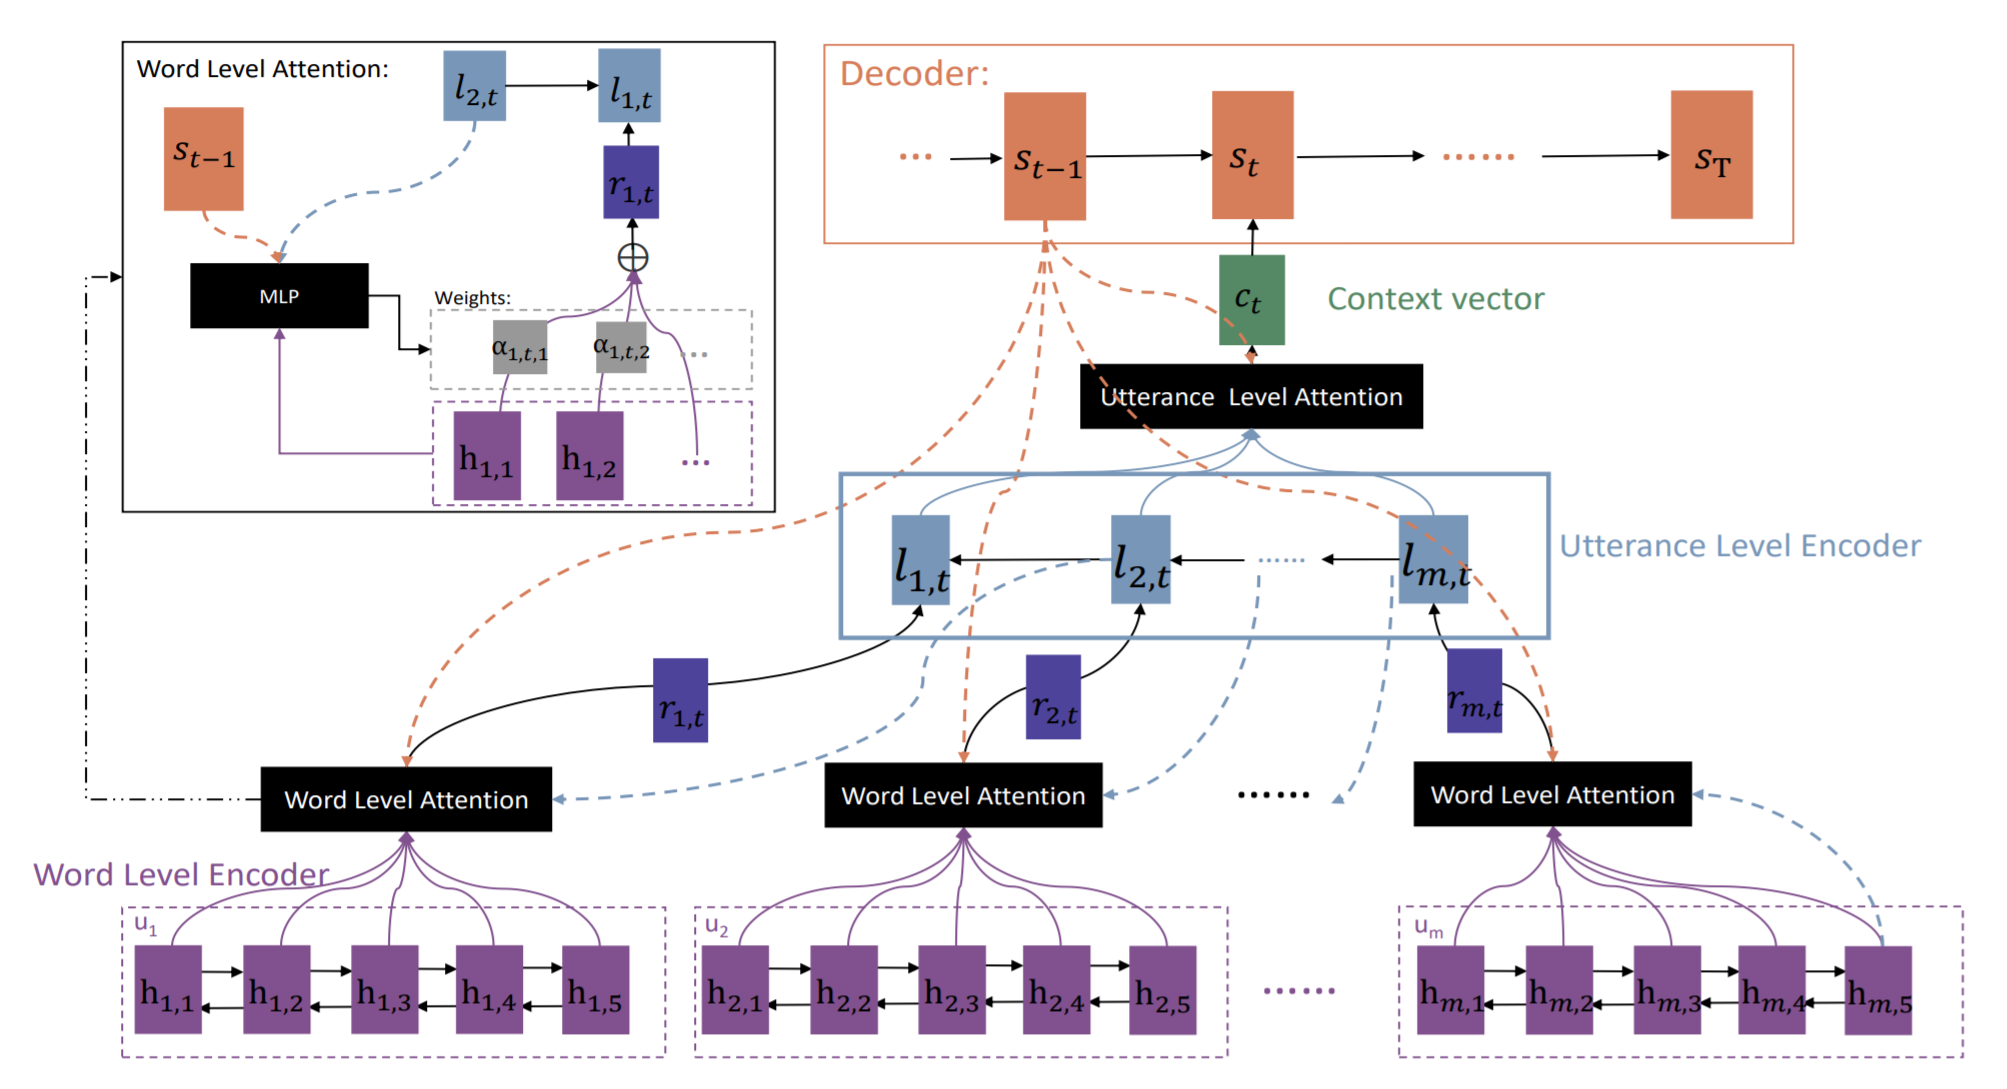
\includegraphics[width=0.9\textwidth]{pics/hran.png}
	\caption{The Hierarchical Recurrent Attention Network \cite{Xing:2017}}
\end{figure}




\subsubsection{Task-Oriented Approaches} \label{sssec:task}
\subsubsection{Reinforcement Learning} \label{sssec:RL}

\subsubsection{Different Encoder-Decoder Models} \label{sssec:diffencdec}
% don't write about attention is all you need here, because you will describe it in ssec:41

\subsection{Criticism} \label{ssec:problems}
\subsubsection{Datasets}
\subsubsection{The Loss Function}
\subsubsection{Memory}
\subsubsection{Evaluation Metrics} \label{sssec:metrics}
% show graphs of how badly standard metrics correlate

\subsection{Summary} \label{ssec:summary}
    

\newpage\section{Experiments} \label{sec:experiments}
\subsection{The Tranformer Model} \label{ssec:41}
\subsection{Datasets} \label{ssec:42}
\subsection{Training Details} \label{ssec:43}

\newpage\section{Results} \label{sec:results}
\subsection{Quantitative Analysis} \label{ssec:51}
\subsection{Qualitative Analysis} \label{ssec:52}

\newpage\section{Future Work} \label{sec:future}
\subsection{Ideas Towards Solving The Loss Function Issue} \label{ssec:61}
\subsection{Temporal Conditioning and Memory} \label{ssec:62}
\subsection{Additional Ideas} \label{ssec:63}

\newpage\section{Conclusion} \label{sec:conclusion}


\bibliographystyle{apalike}
\newpage\bibliography{chatbots}
\end{document}
